\documentclass{beamer}

\usetheme{Madrid}
\usepackage{graphicx}
\usepackage{multimedia}
\usepackage{tabularx}
\usepackage{subfig}
\usepackage{amsmath}
\usepackage{comment}
\usepackage{tikz}
\usepackage{tikz-qtree}
\usetikzlibrary{matrix}

\tikzset{edge from parent/.style=
{draw, edge from parent path={(\tikzparentnode.south)
-- +(0,-8pt)
-| (\tikzchildnode)}},
blank/.style={draw=none}}





\title{Achieving Seamlessness in Multi-Projector based Tiled Display using Camera Feedback}
\author{Pranav Kant Gaur}
\institute{Graphics and Visualization section}

\date{\today}

\begin{document}

\begin{frame}
\titlepage
\end{frame}





%//////////////////////////////////////////////////////////////////////////////////////////////////////////////////////////////////
\begin{frame}
\frametitle{Agenda}
\begin{enumerate}
\item Objective 
\item Motivation
\item Challenges
\item Why not a commercial solution?
\item Approaches tried
\item Followed approach
\item System setup
\item Algorithm 
\item Contributions
\item Results
\item Issues
\end{enumerate}
\end{frame}
%//////////////////////////////////////////////////////////////////////////////////////////////////////////////////////////////////

%//////////////////////////////////////////////////////////////////////////////////////////////////////////////////////////////////
\begin{frame}
\frametitle{Objective}
%Given an arbitrarily arranged grid of projectors projecting at arbitrary positions onto the screen, find the region in each projector image buffer where if the original image is mapped onto will result in a seamless rectangular projection region on the screen.\newline
%In short, 
%ADD UNALIGNED=> ALIGNED ??????????????????????
%Given an arbitrarily arranged grid of projectors projecting at arbitrary positions onto the screen, how to manipulate each projector image so that projected content is \textit{seamless} across the adjacent projectors. \textb{ADD FIGURE!!!!}
We want to create a large image on the projection screen by combining images projected by multiple projectors.

\begin{figure}
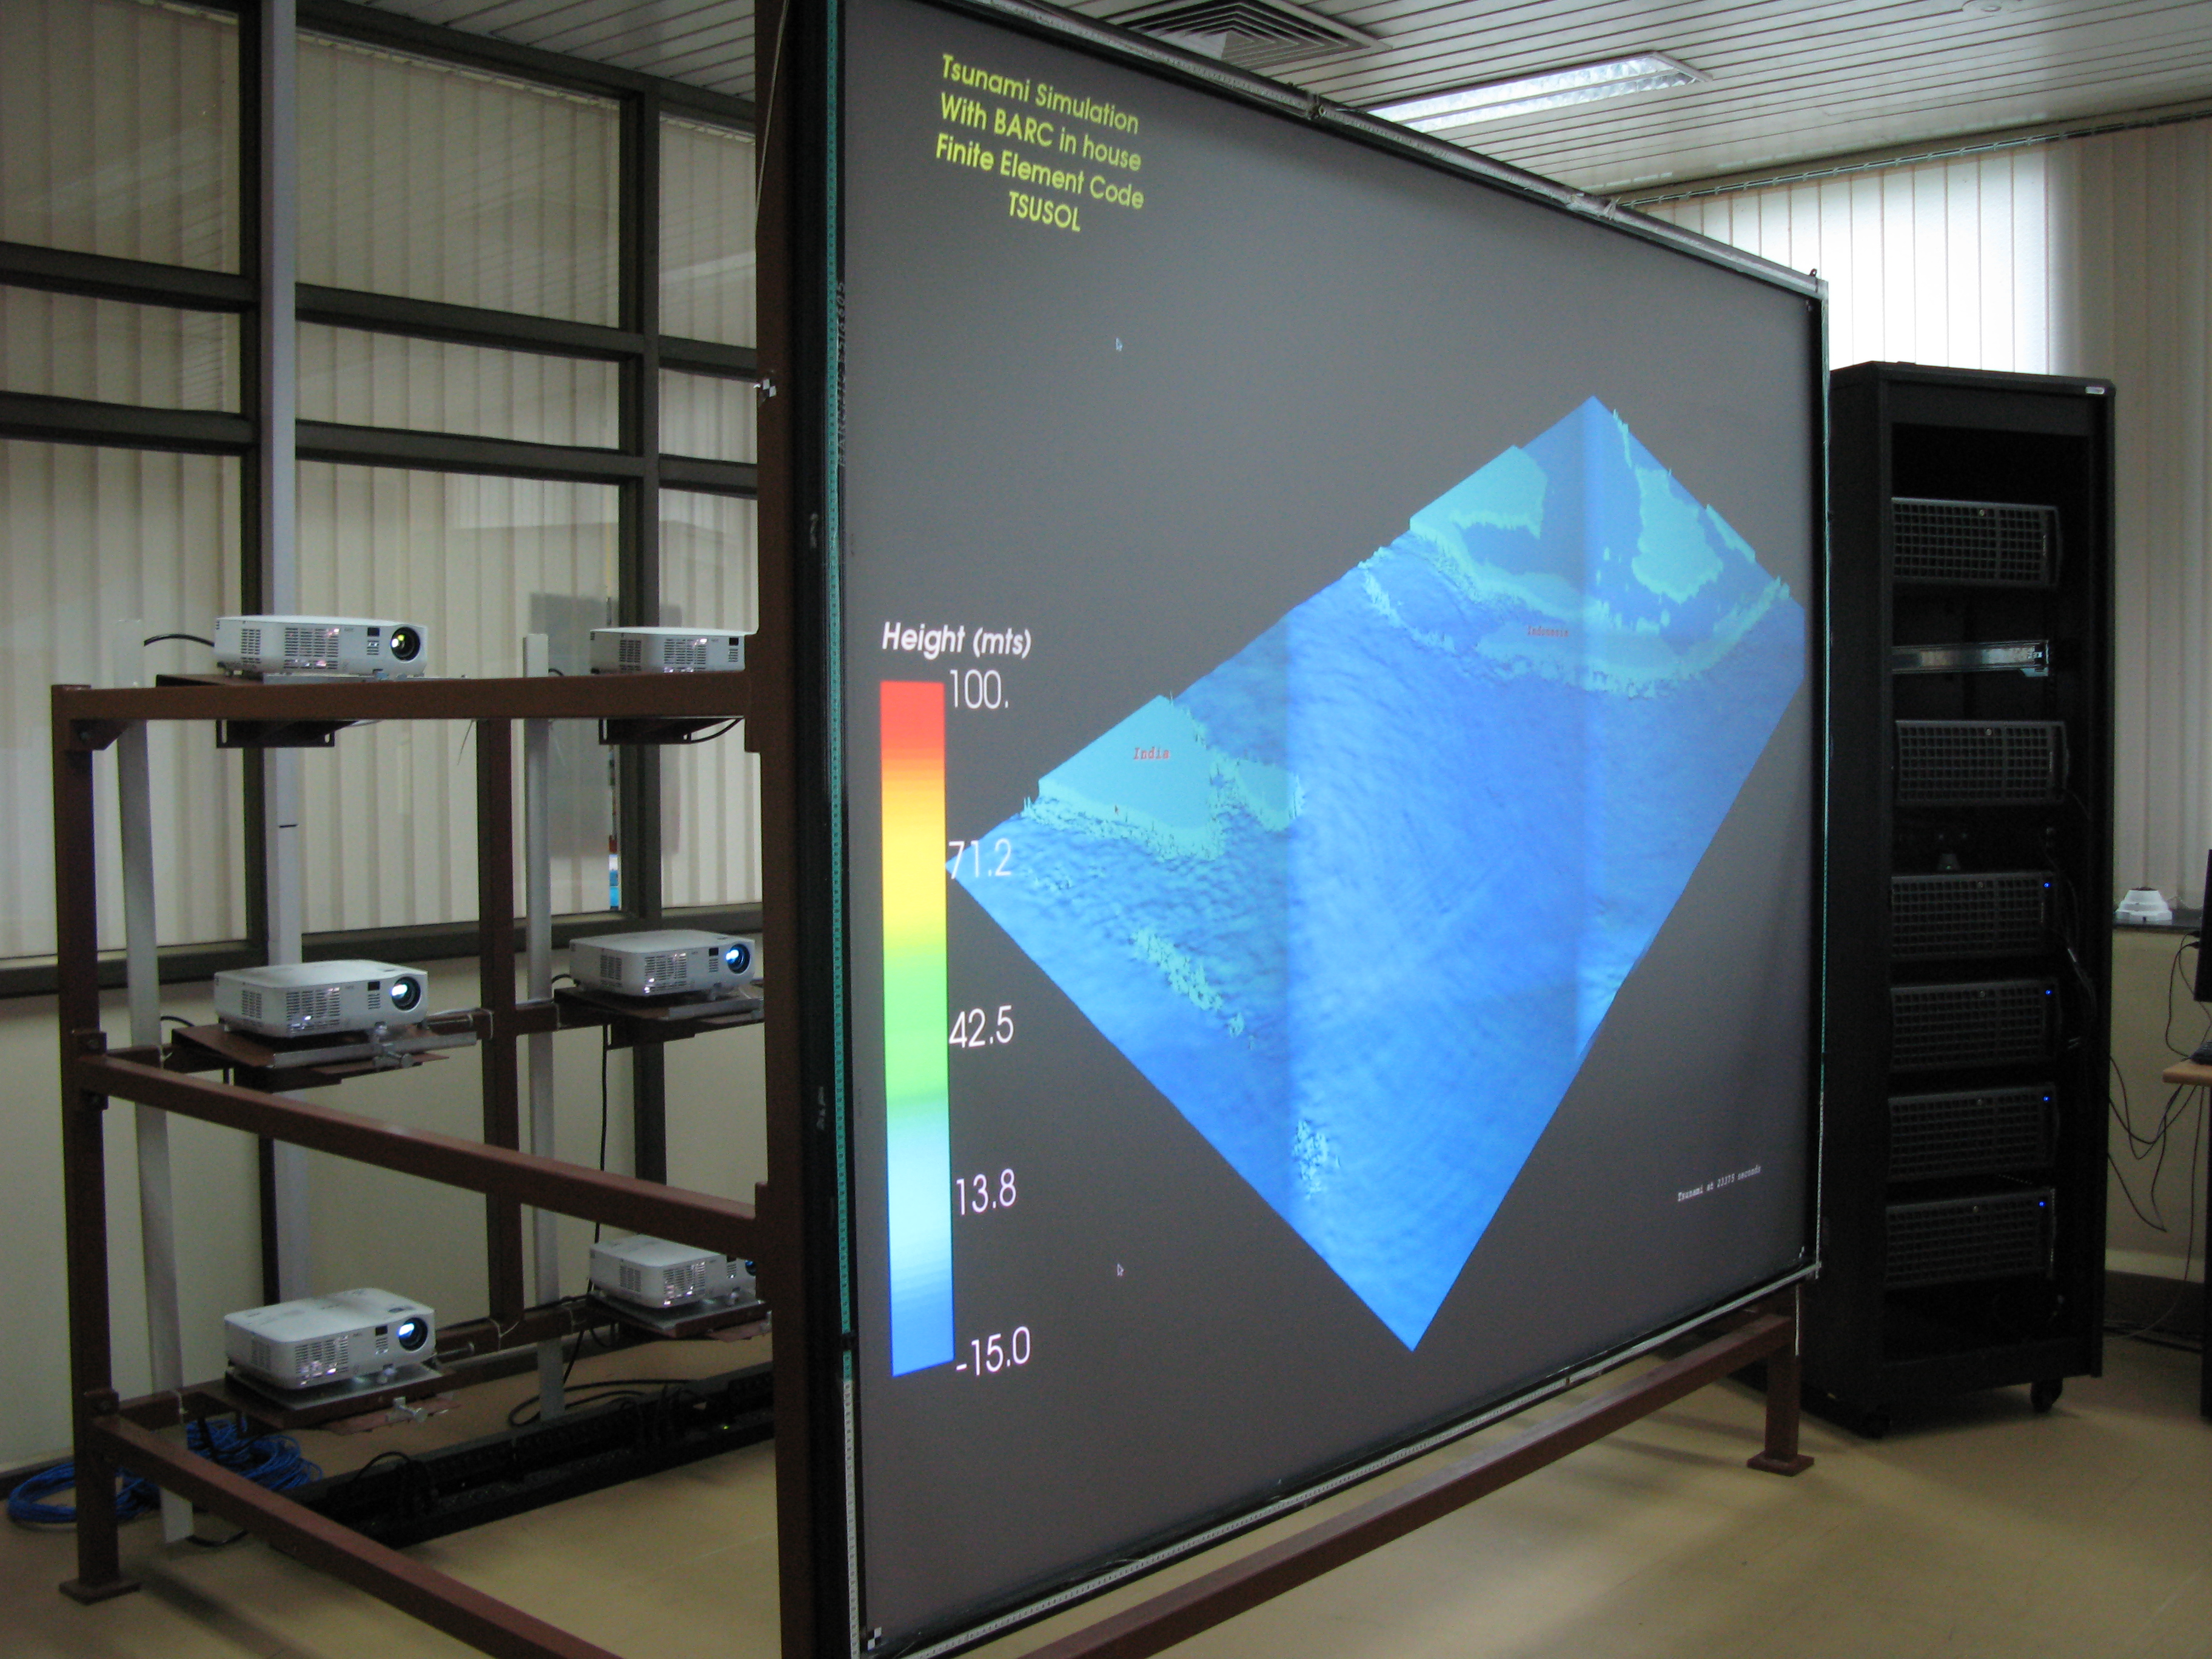
\includegraphics[width=6.0cm,height=4cm]{figures/system_setup.jpg}
\caption{Multiprojector tiled display}
\end{figure}

\end{frame}
%//////////////////////////////////////////////////////////////////////////////////////////////////////////////////////////////////

%//////////////////////////////////////////////////////////////////////////////////////////////////////////////////////////////////
\begin{frame}
\frametitle{Motivation}
\begin{itemize}
\item Why \textit{Tiled}?\newline
An image with spatial resolution higher than that \textit{perceivable} by human eye cannot be visualized without reducing its resolution. We can achieve this by spatially \textit{stretching} the content.
\item Why \textit{Multiprojector}?\newline
Seams of monitors used in our earlier Tiled display system were \textit{distracting}. Projectors do not pose such limitation.
\end{itemize}
\end{frame}

%//////////////////////////////////////////////////////////////////////////////////////////////////////////////////////////////////
%\begin{frame}{Existing solutions}
%\begin{enumerate}
%\item Manual 
%\begin{enumerate}
%\item Keystone correction
%\item Interactive image manipulation
%\end{enumerate}
%\item Automatic
%\begin{enumerate}
%\item Homography 
%\item Structured light 
%\item Brown's approach
%\item Raskar's approach
%\end{enumerate}
%\end{enumerate}
%\end{frame}

%//////////////////////////////////////////////////////////////////////////////////////////////////////////////////////////////////

\begin{frame}{Challenges}
\begin{enumerate}
\item Perspective distortion removal
\begin{figure}
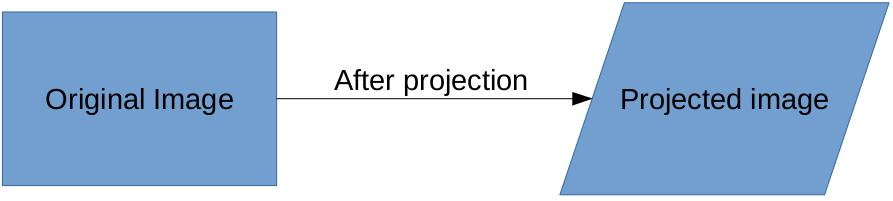
\includegraphics[width=8cm,height=2.5cm]{figures/distortion_prob.jpg}
\end{figure} 
\item Geometric continuity of projected content
\begin{figure}
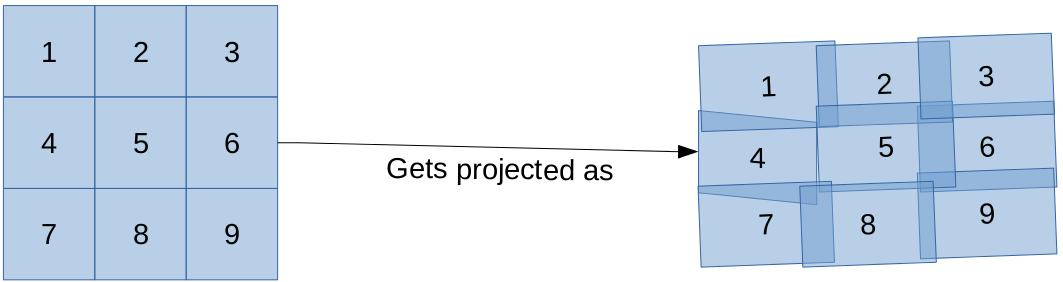
\includegraphics[width=8cm, height=2.5cm]{figures/continuity_prob.jpg}
\end{figure}
\item Handling intensity in overlap region
\end{enumerate}
\end{frame}

%//////////////////////////////////////////////////////////////////////////////////////////////////////////////////////////////////

\begin{frame}{Why not a commercial solution?}

\underline{Our requirements}:
\begin{itemize}
\item Configurable
\item Portable
\item Control over trouble-shooting
\end{itemize}

\underline{Limitations of current commercial systems}:
\begin{itemize}
\item Software packages:
\begin{itemize}
\item Limited support for cameras used for calibration.
\item Limited support for Graphics cards. 
\item Not open source, some vendors provide API's only.
\item Do not work with Linux.
\end{itemize}
\end{itemize}
\end{frame}

%//////////////////////////////////////////////////////////////////////////////////////////////////////////////////////////////////

\begin{frame}{Commercial systems(contd.)}
\begin{itemize}
\item Hardware + Software products:
\begin{itemize}
\item Separate image processing box for generating seamless image.
\item Factory configured, support for configured is very limited.
\end{itemize}
\end{itemize}

\begin{figure}
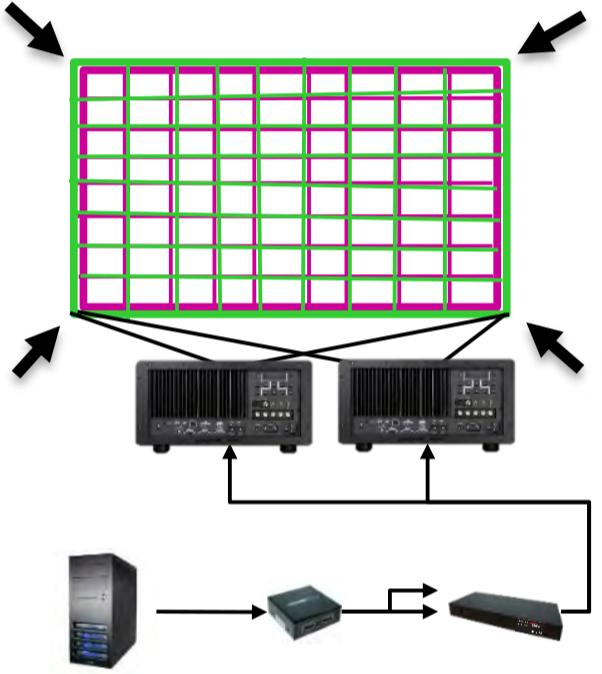
\includegraphics[width=6cm,height=4.5cm]{figures/commercial.jpg}
\caption{Commercial System, Image source: Optoma USA}
\end{figure}

\end{frame}

%//////////////////////////////////////////////////////////////////////////////////////////////////////////////////////////////////
%\begin{frame}{Approaches tried}
%\underline{Didn't solved our purpose}:
%\begin{itemize}
%\item \textbf{Interactive projector alignent(Compiz, Chromium)}:
%\begin{itemize}
%\item Not scalable. Interactive correction of all corners of each projector image
%\item Tedious. Endpoints of adjacent projectors should coincide
%\end{itemize}
%\item \textbf{Fixed region projection(Homography)}:
%\begin{itemize}
%\item Constrains projector placement
%\item Not scalable. Accurate mesurements on the bigger screens are not always practical
%\end{itemize}
%\item \textbf{Automatic projector aligment using Error feedback}:
%\begin{itemize}
%\item Alignment process oscillates when error becomes very low
%\item Can work only for non-overlapping configurations
%\end{itemize}
%\end{itemize}

%\underline{Approach that worked}:
%\begin{itemize}
%\item \textbf{Camera based geometric alignment and edge blending}:
%\begin{itemize}
%\item Completely automatic
%\item Scalable
%\item Projector placement is not constrained
%\end{itemize}
%\end{itemize}
%\end{frame}



%////////////////////////////////////////////////////////////////////////////////////////////////////////////////////////////////i/


%\begin{frame}[label=concept]
%\frametitle{Followed approach}
%\begin{enumerate}
%\item Geometric alignment
%\begin{enumerate}
%\item For each projector, determine distortion introduced by it in the projected image on screen.
%\item Apply inverse of this distortion to the projector image to recover geometrically continuous projection across neighboring projectors.
%\end{enumerate}
%\item Edge blending
%\begin{enumerate}
%\item Determine overlapping region between neighbouring projectors
%\item Attenuate intensity of pixels in that region for all overlapping projectors so that their overlap does not create \textit{bright} junction between them
%\end{enumerate}
%\end{enumerate}
%\end{frame}

%//////////////////////////////////////////////////////////////////////////////////////////////////////////////////////////////////

\begin{frame}
\frametitle{Approaches tried}
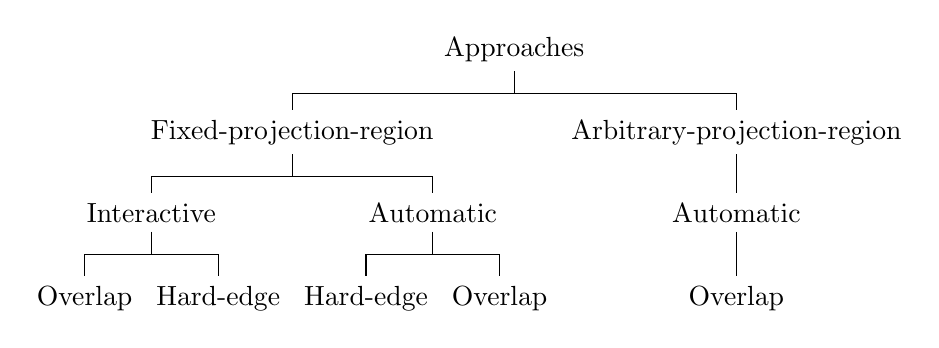
\begin{tikzpicture}
\Tree[.Approaches [.Fixed-projection-region [.Interactive  Overlap Hard-edge ] [.Automatic Hard-edge Overlap ] ] [.Arbitrary-projection-region [.Automatic Overlap ] ] ]         
\end{tikzpicture}

\begin{figure}
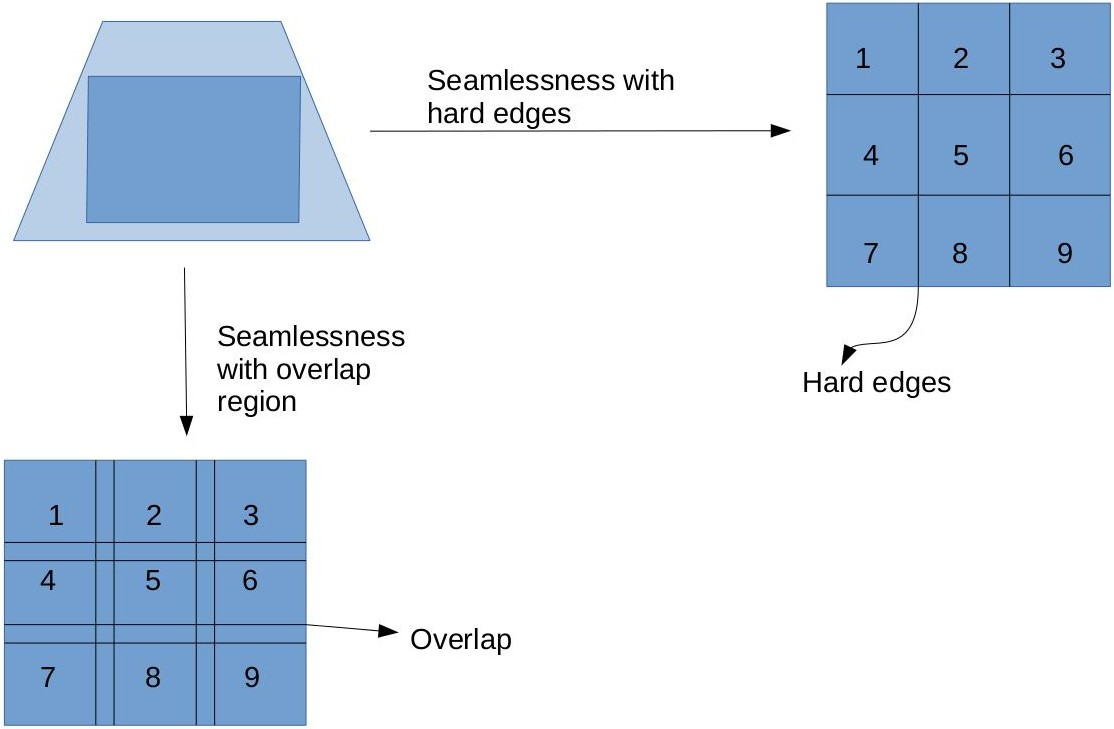
\includegraphics[width=6cm, height=4cm]{figures/hard_overlap.jpg}
\end{figure}
\end{frame}

%//////////////////////////////////////////////////////////////////////////////////////////////////////////////////////////////////


\begin{frame}{Followed approach}
\begin{itemize}
\item Removing perspective distortion
\begin{figure}
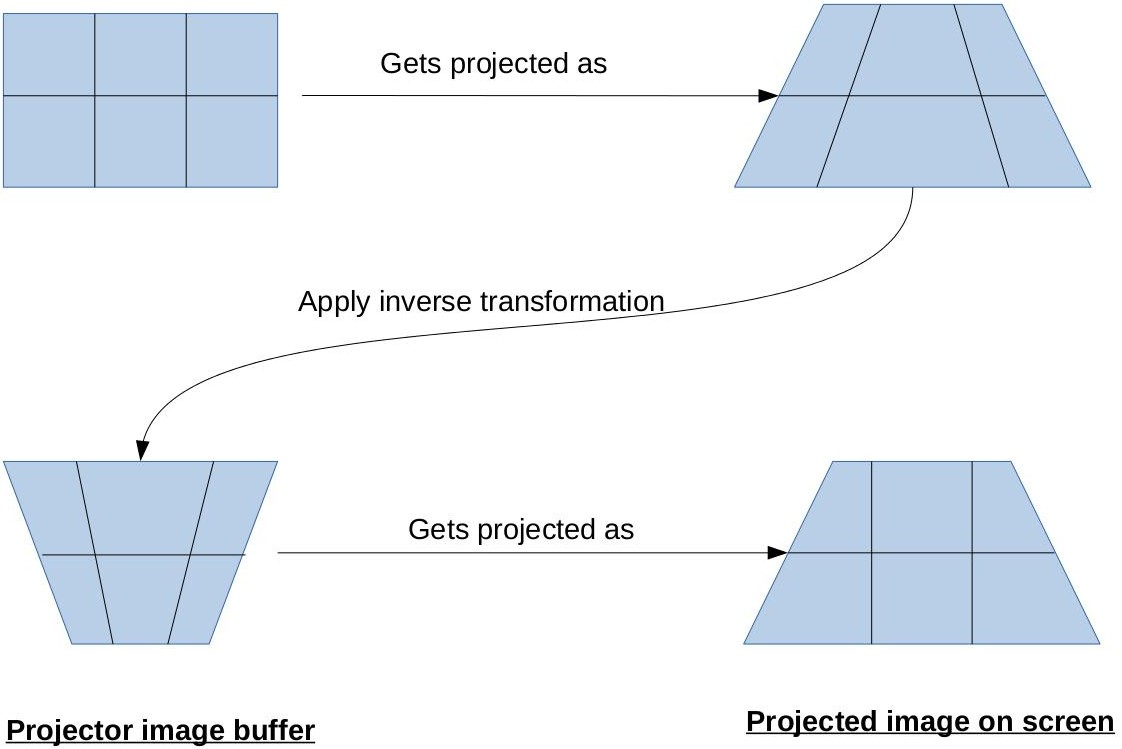
\includegraphics[width=7cm, height=5cm]{figures/distort_sol.jpg}
\end{figure}
\end{itemize}
\end{frame}

%//////////////////////////////////////////////////////////////////////////////////////////////////////////////////////////////////

\begin{frame}{Followed approach(contd.)}
\begin{itemize}
\item Ensuring geometric continuity
\begin{figure}
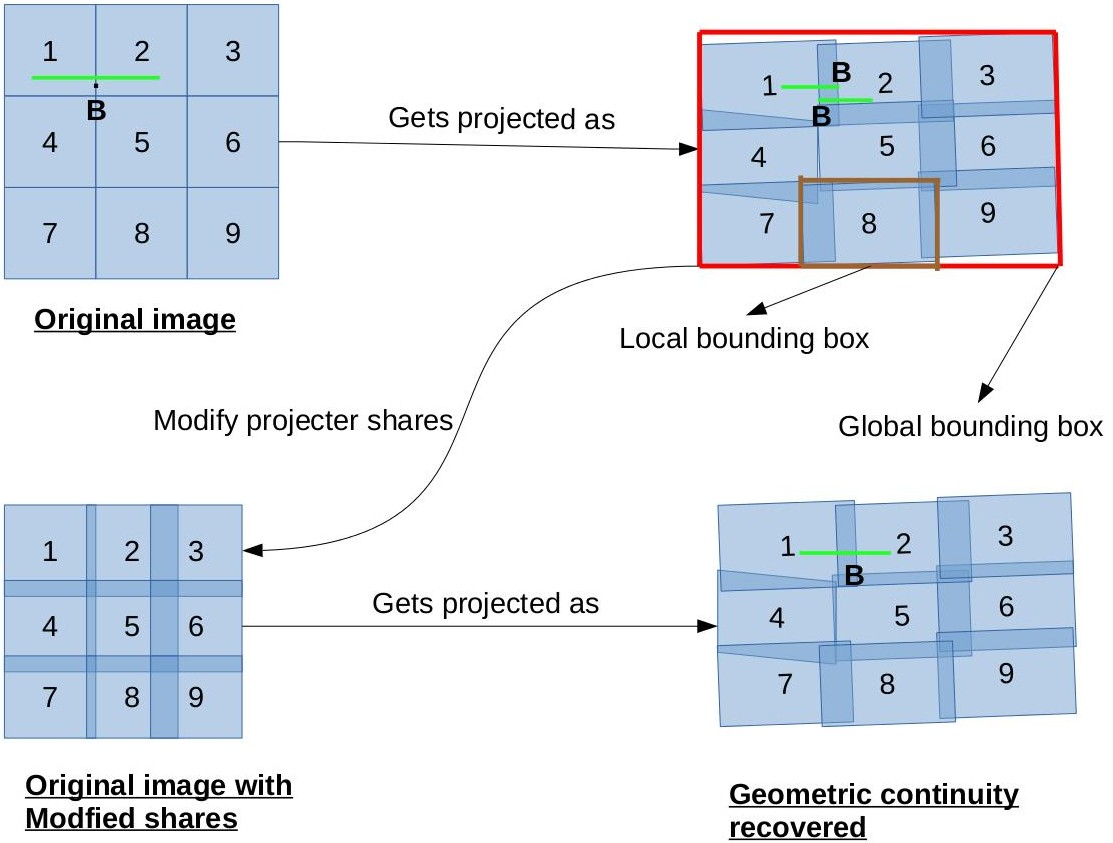
\includegraphics[width=8cm,height=6cm]{figures/continuity_better.jpg}
\end{figure}
\end{itemize}
\end{frame}


%//////////////////////////////////////////////////////////////////////////////////////////////////////////////////////////////////

\begin{frame}{Followed approach(contd.)}
\begin{itemize}
\item Handling image intensity at the overlap region
\begin{figure}
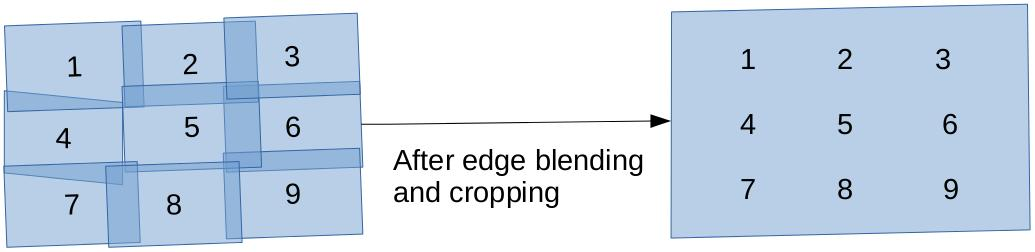
\includegraphics[width=9cm,height=3cm]{figures/blending.jpg}
\end{figure}
\end{itemize}
\end{frame}
\begin{frame}
\frametitle{System setup}
Developed system has:
\begin{itemize}
\item 3X3 grid of projectors
\item Rear projection screen
\item 1 digital camera
\item Workstations arranged in master-slave configuration
\end{itemize}

\begin{figure}
\centering
\begin{tabularx}{\linewidth}{@{}cXX@{}}
\begin{tabular}{c c}
\hspace{0.5cm}\subfloat[System setup]{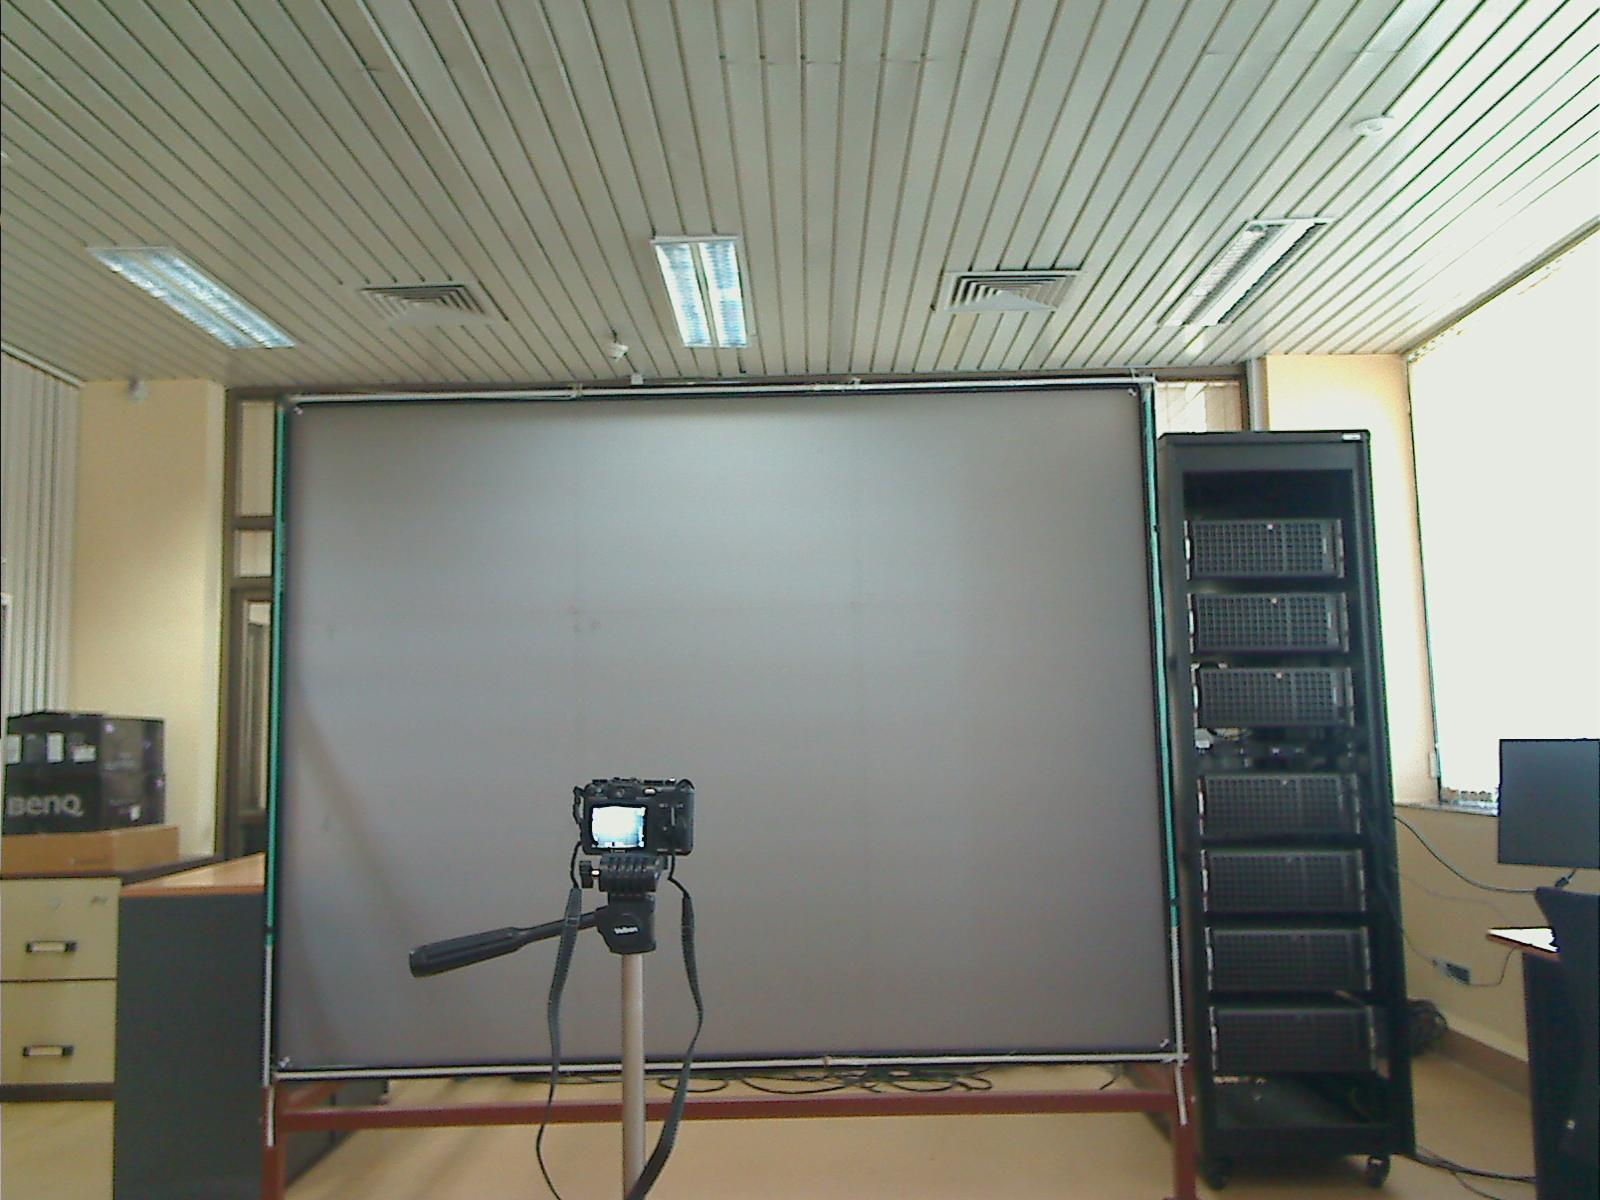
\includegraphics[width=4.5cm,height=3cm]{figures/setup.jpg}} & 
\subfloat[Projector-array behind the projection screen]{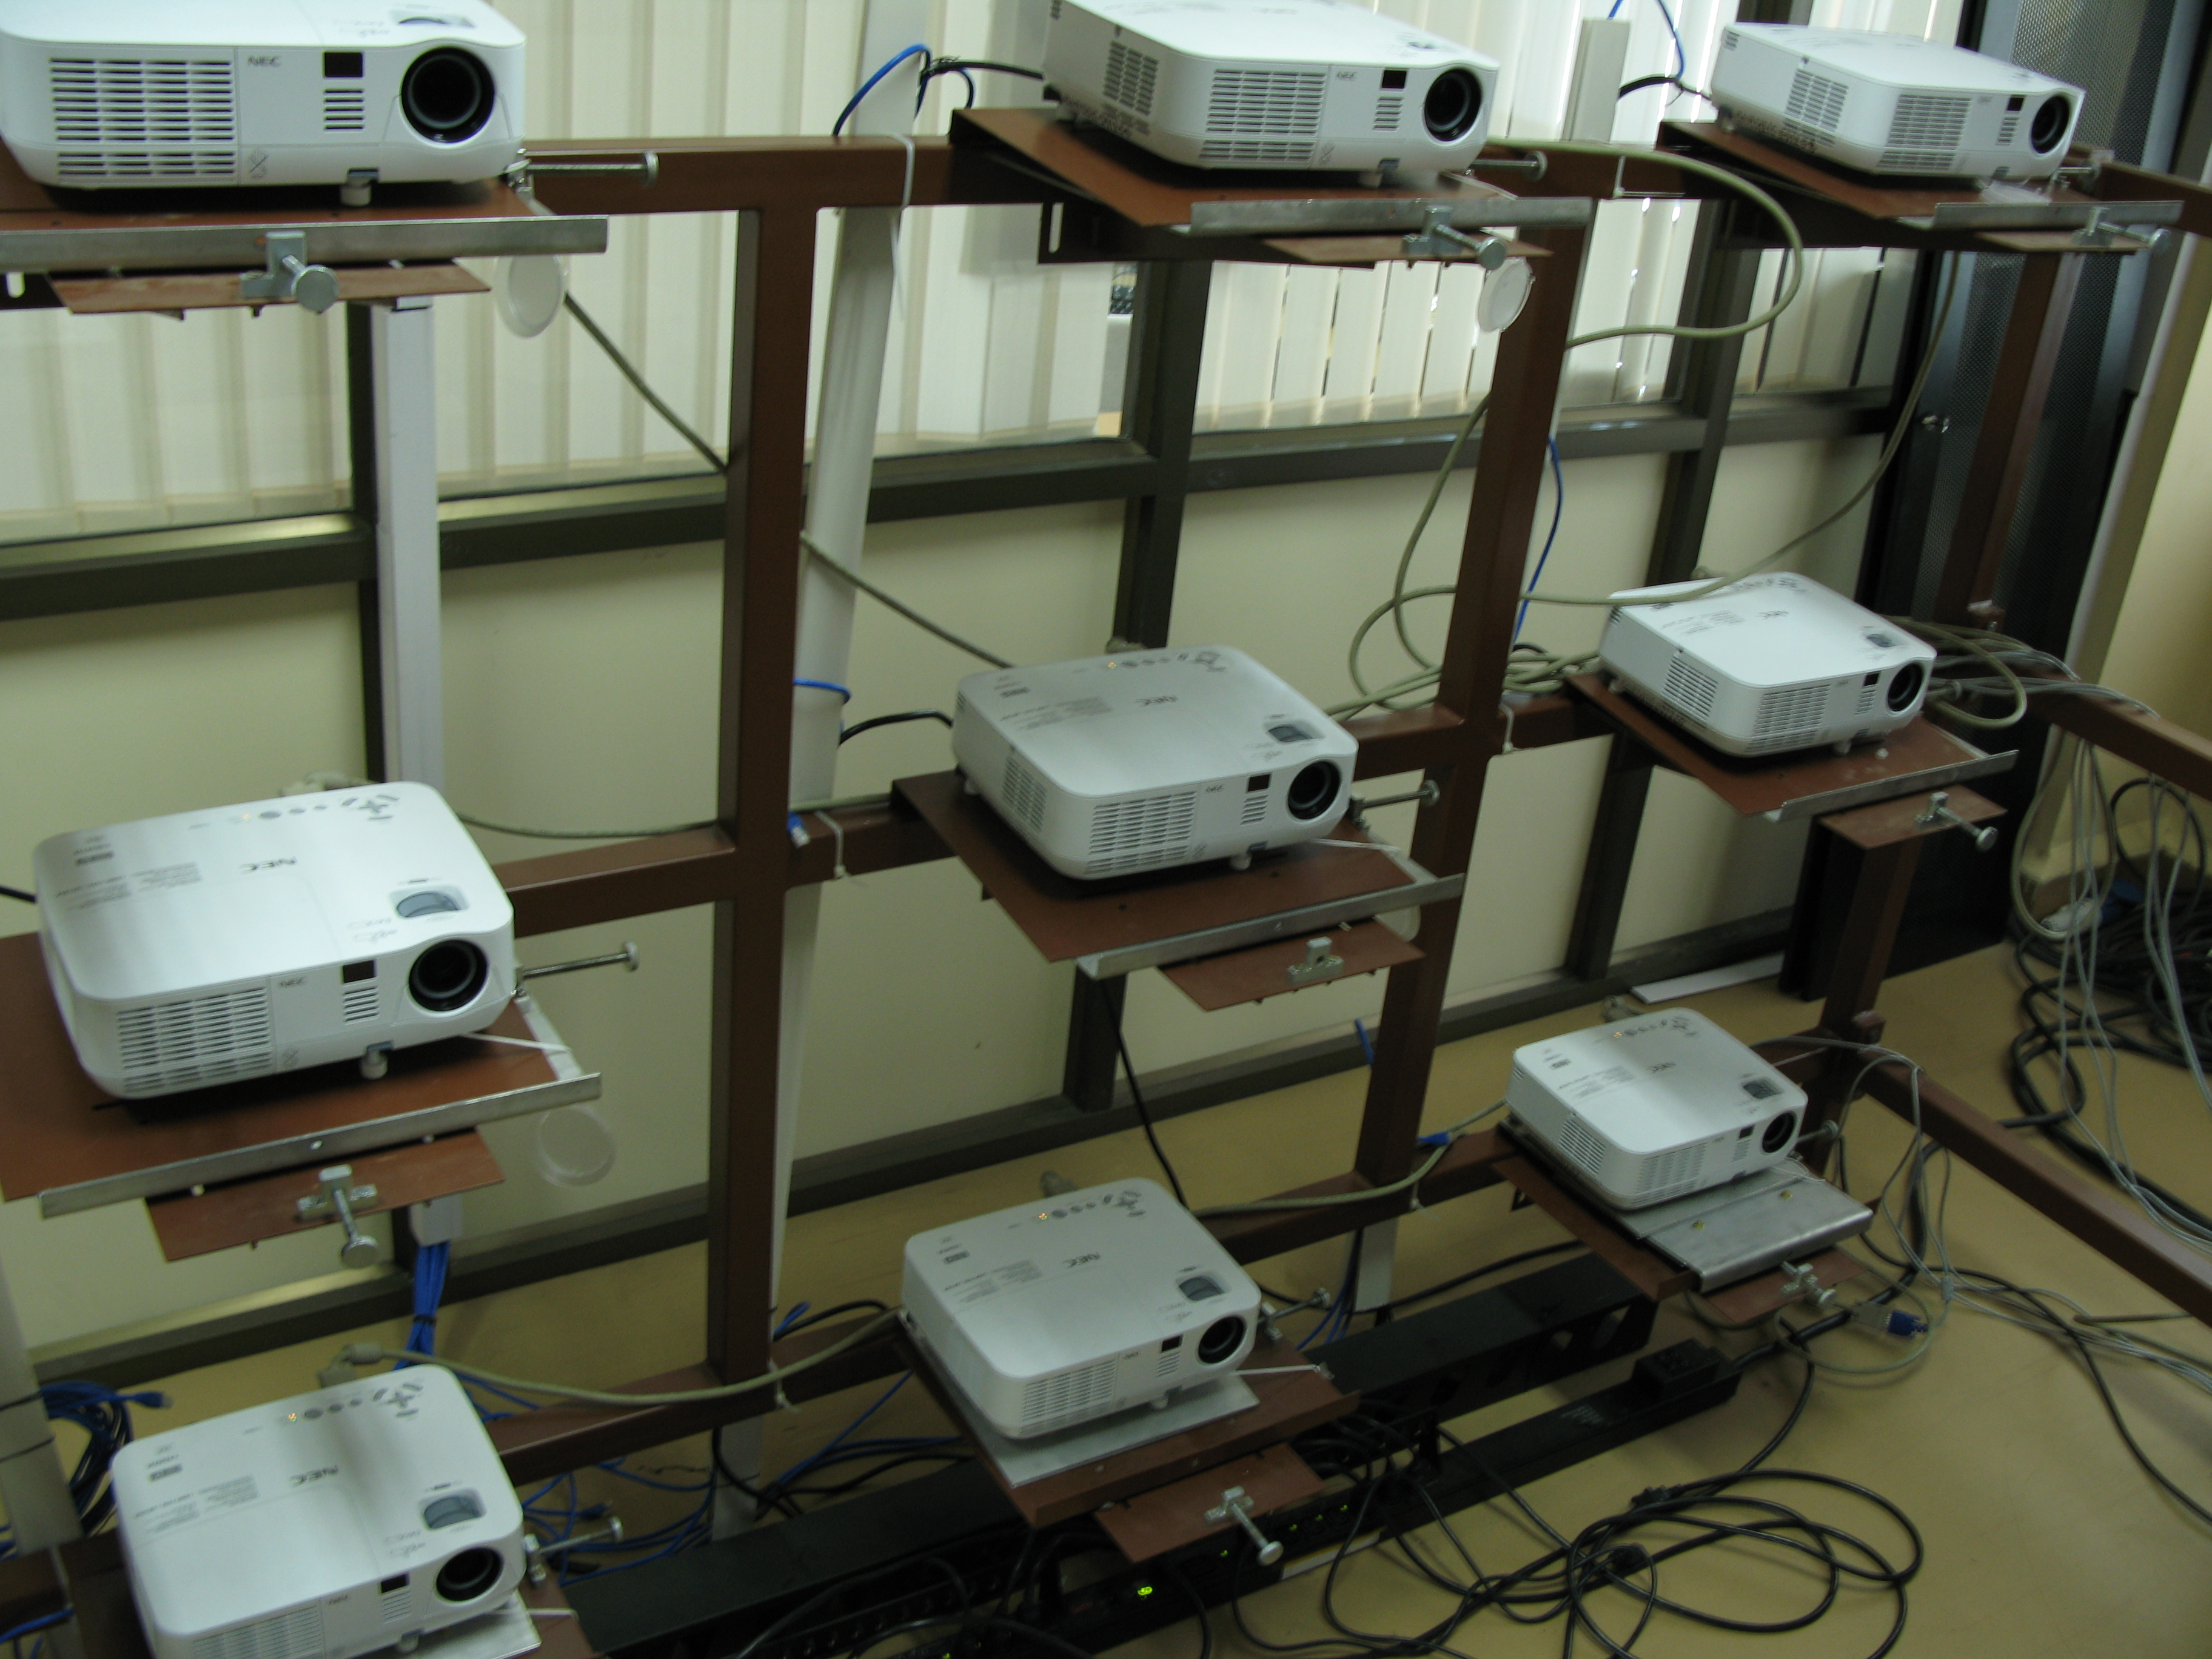
\includegraphics[width=4.5cm,height=3cm]{figures/projs.jpg}} \\
\end{tabular}
\end{tabularx}
\end{figure}

\end{frame}

%//////////////////////////////////////////////////////////////////////////////////////////////////////////////////////////////////
\begin{frame}{Algorithm}
\begin{itemize}
\item Based on paper `A practical and flexible tiled
display system' by M.S. Brown and W.B. Seales.
\item \underline{Algorithm overview}:
\begin{enumerate}
\item Relation between Camera and screen coordinate system is determined.
\item Each projector projects a checkerboard, camera captures the view and checkerboard corners are detected.
\item For each projector, corresponding detected corners are addressed in a local bounding box. 
\item Global bounding box containing all local bounding boxes are computed. 
\item Overlap between adjacent projectors is determined. 
\end{enumerate}
\end{itemize}
\end{frame}

%//////////////////////////////////////////////////////////////////////////////////////////////////////////////////////////////////

\begin{frame}
\frametitle{Algorithm(contd.)}
\framesubtitle{Compute screen to camera relation}
\begin{itemize}
\item We want \hyperlink{concept}{\textit{Geometrically aligned}} and \hyperlink{concept}{\textit{seamless}} content on projection screen.
\item Camera is just a \textit{feedback device}.
\item All later calculations are performed in screen-coordinate system.
\end{itemize}

\begin{figure}
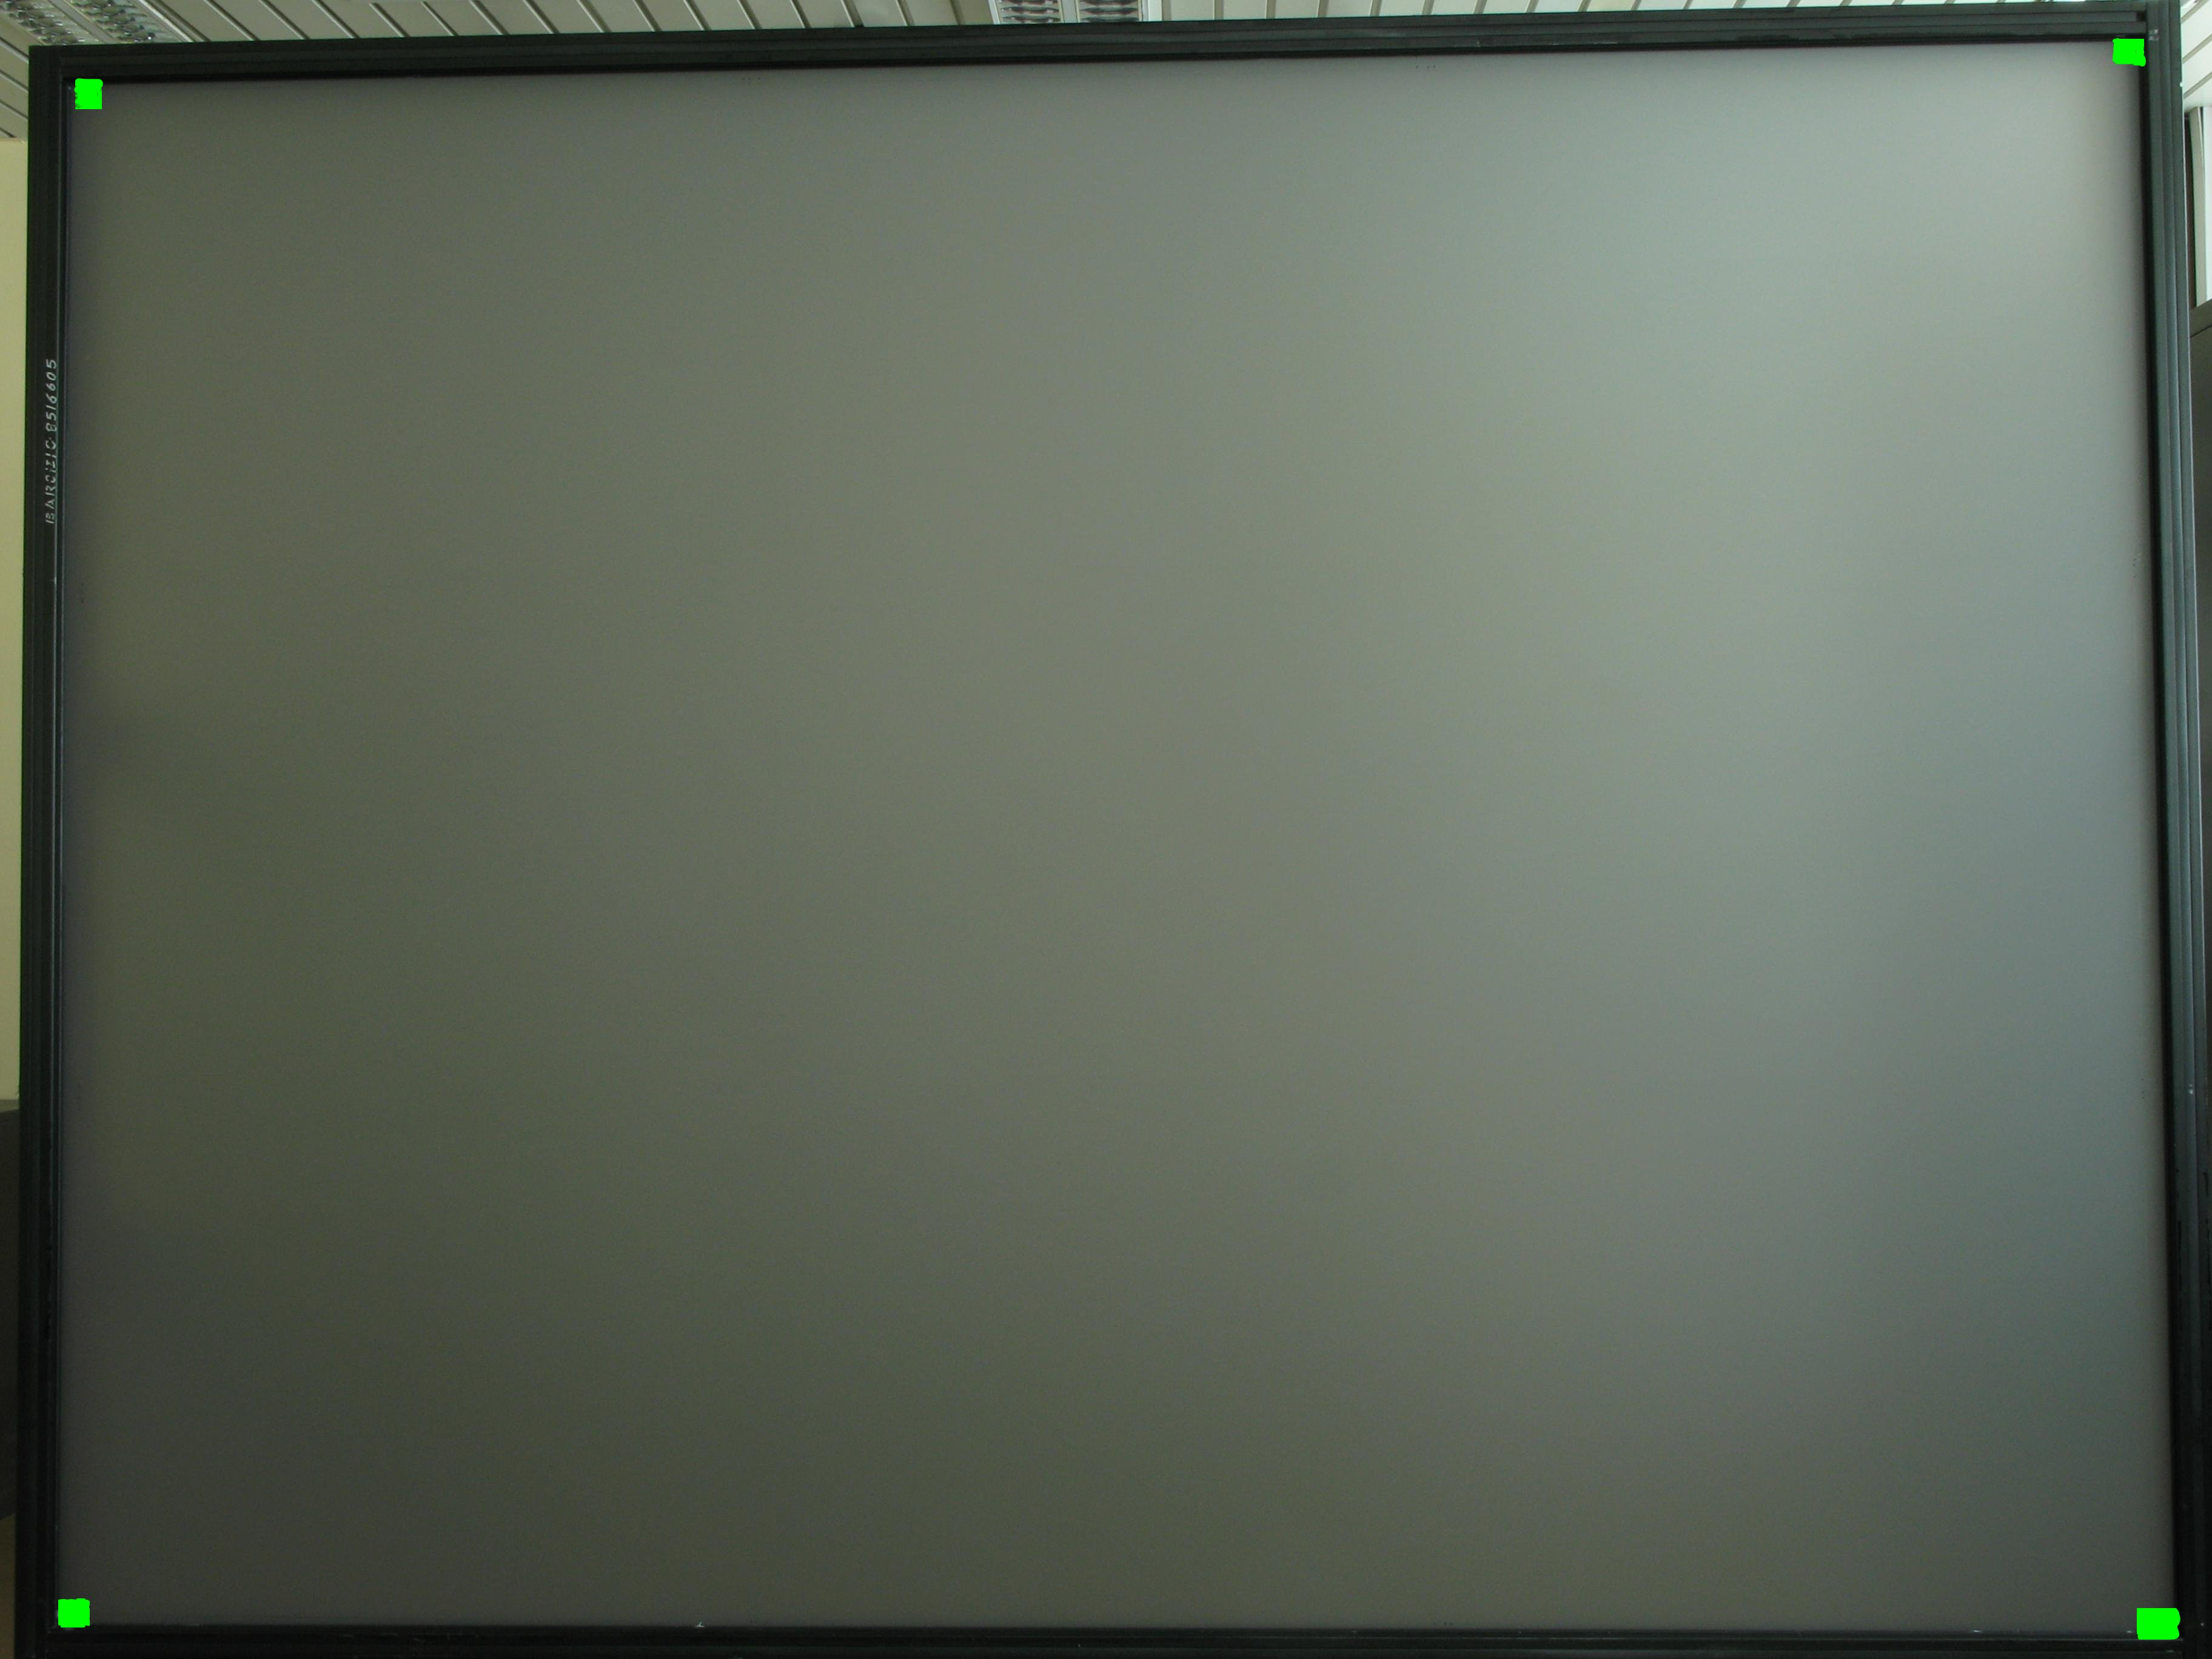
\includegraphics[width=6cm, height = 4cm]{figures/debug_image_features.jpg}
\caption{View from camera}
\end{figure}
\end{frame}

%//////////////////////////////////////////////////////////////////////////////////////////////////////////////////////////////////

\begin{frame}
\frametitle{Algorithm(contd.): Remove perspective distortion}
\framesubtitle{Project and detect features for each projector}
Detected features are mapped to screen coordinate system.

\begin{figure}
\centering
\begin{tabularx}{\linewidth}{@{}cXX@{}}
\begin{tabular}{c c}
\hspace{0.5cm}\subfloat[Projected features]{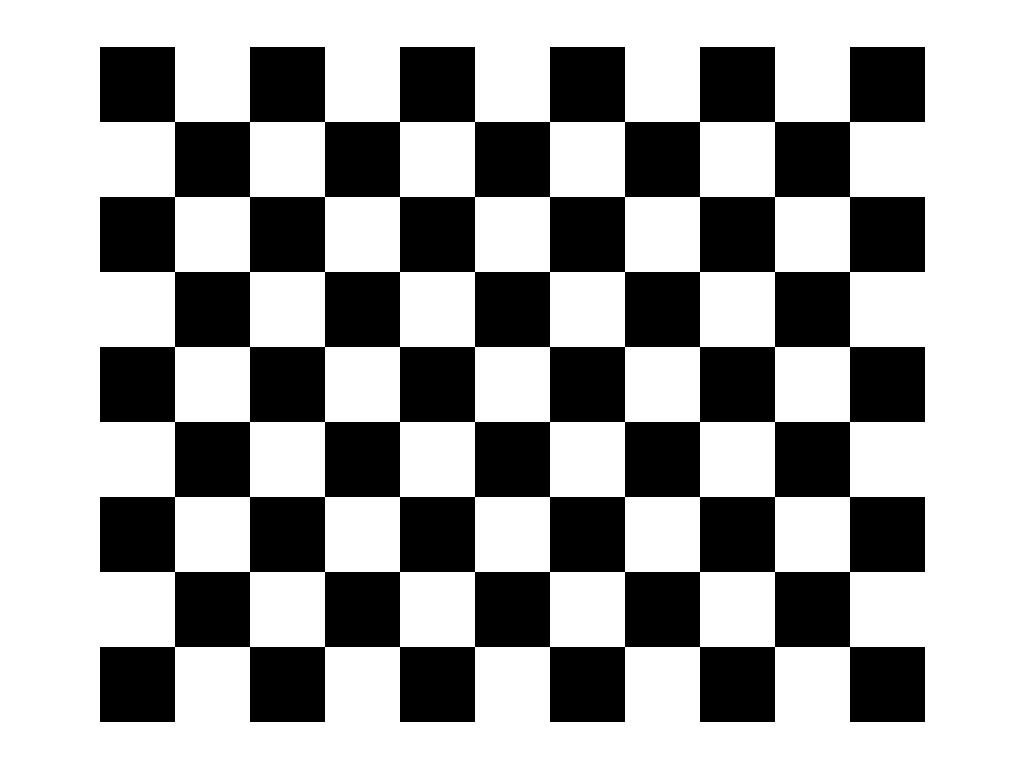
\includegraphics[width=4.5cm,height=3cm]{figures/checkerboard.jpg}} &
\subfloat[Low exposure image of detected features for the central projector]{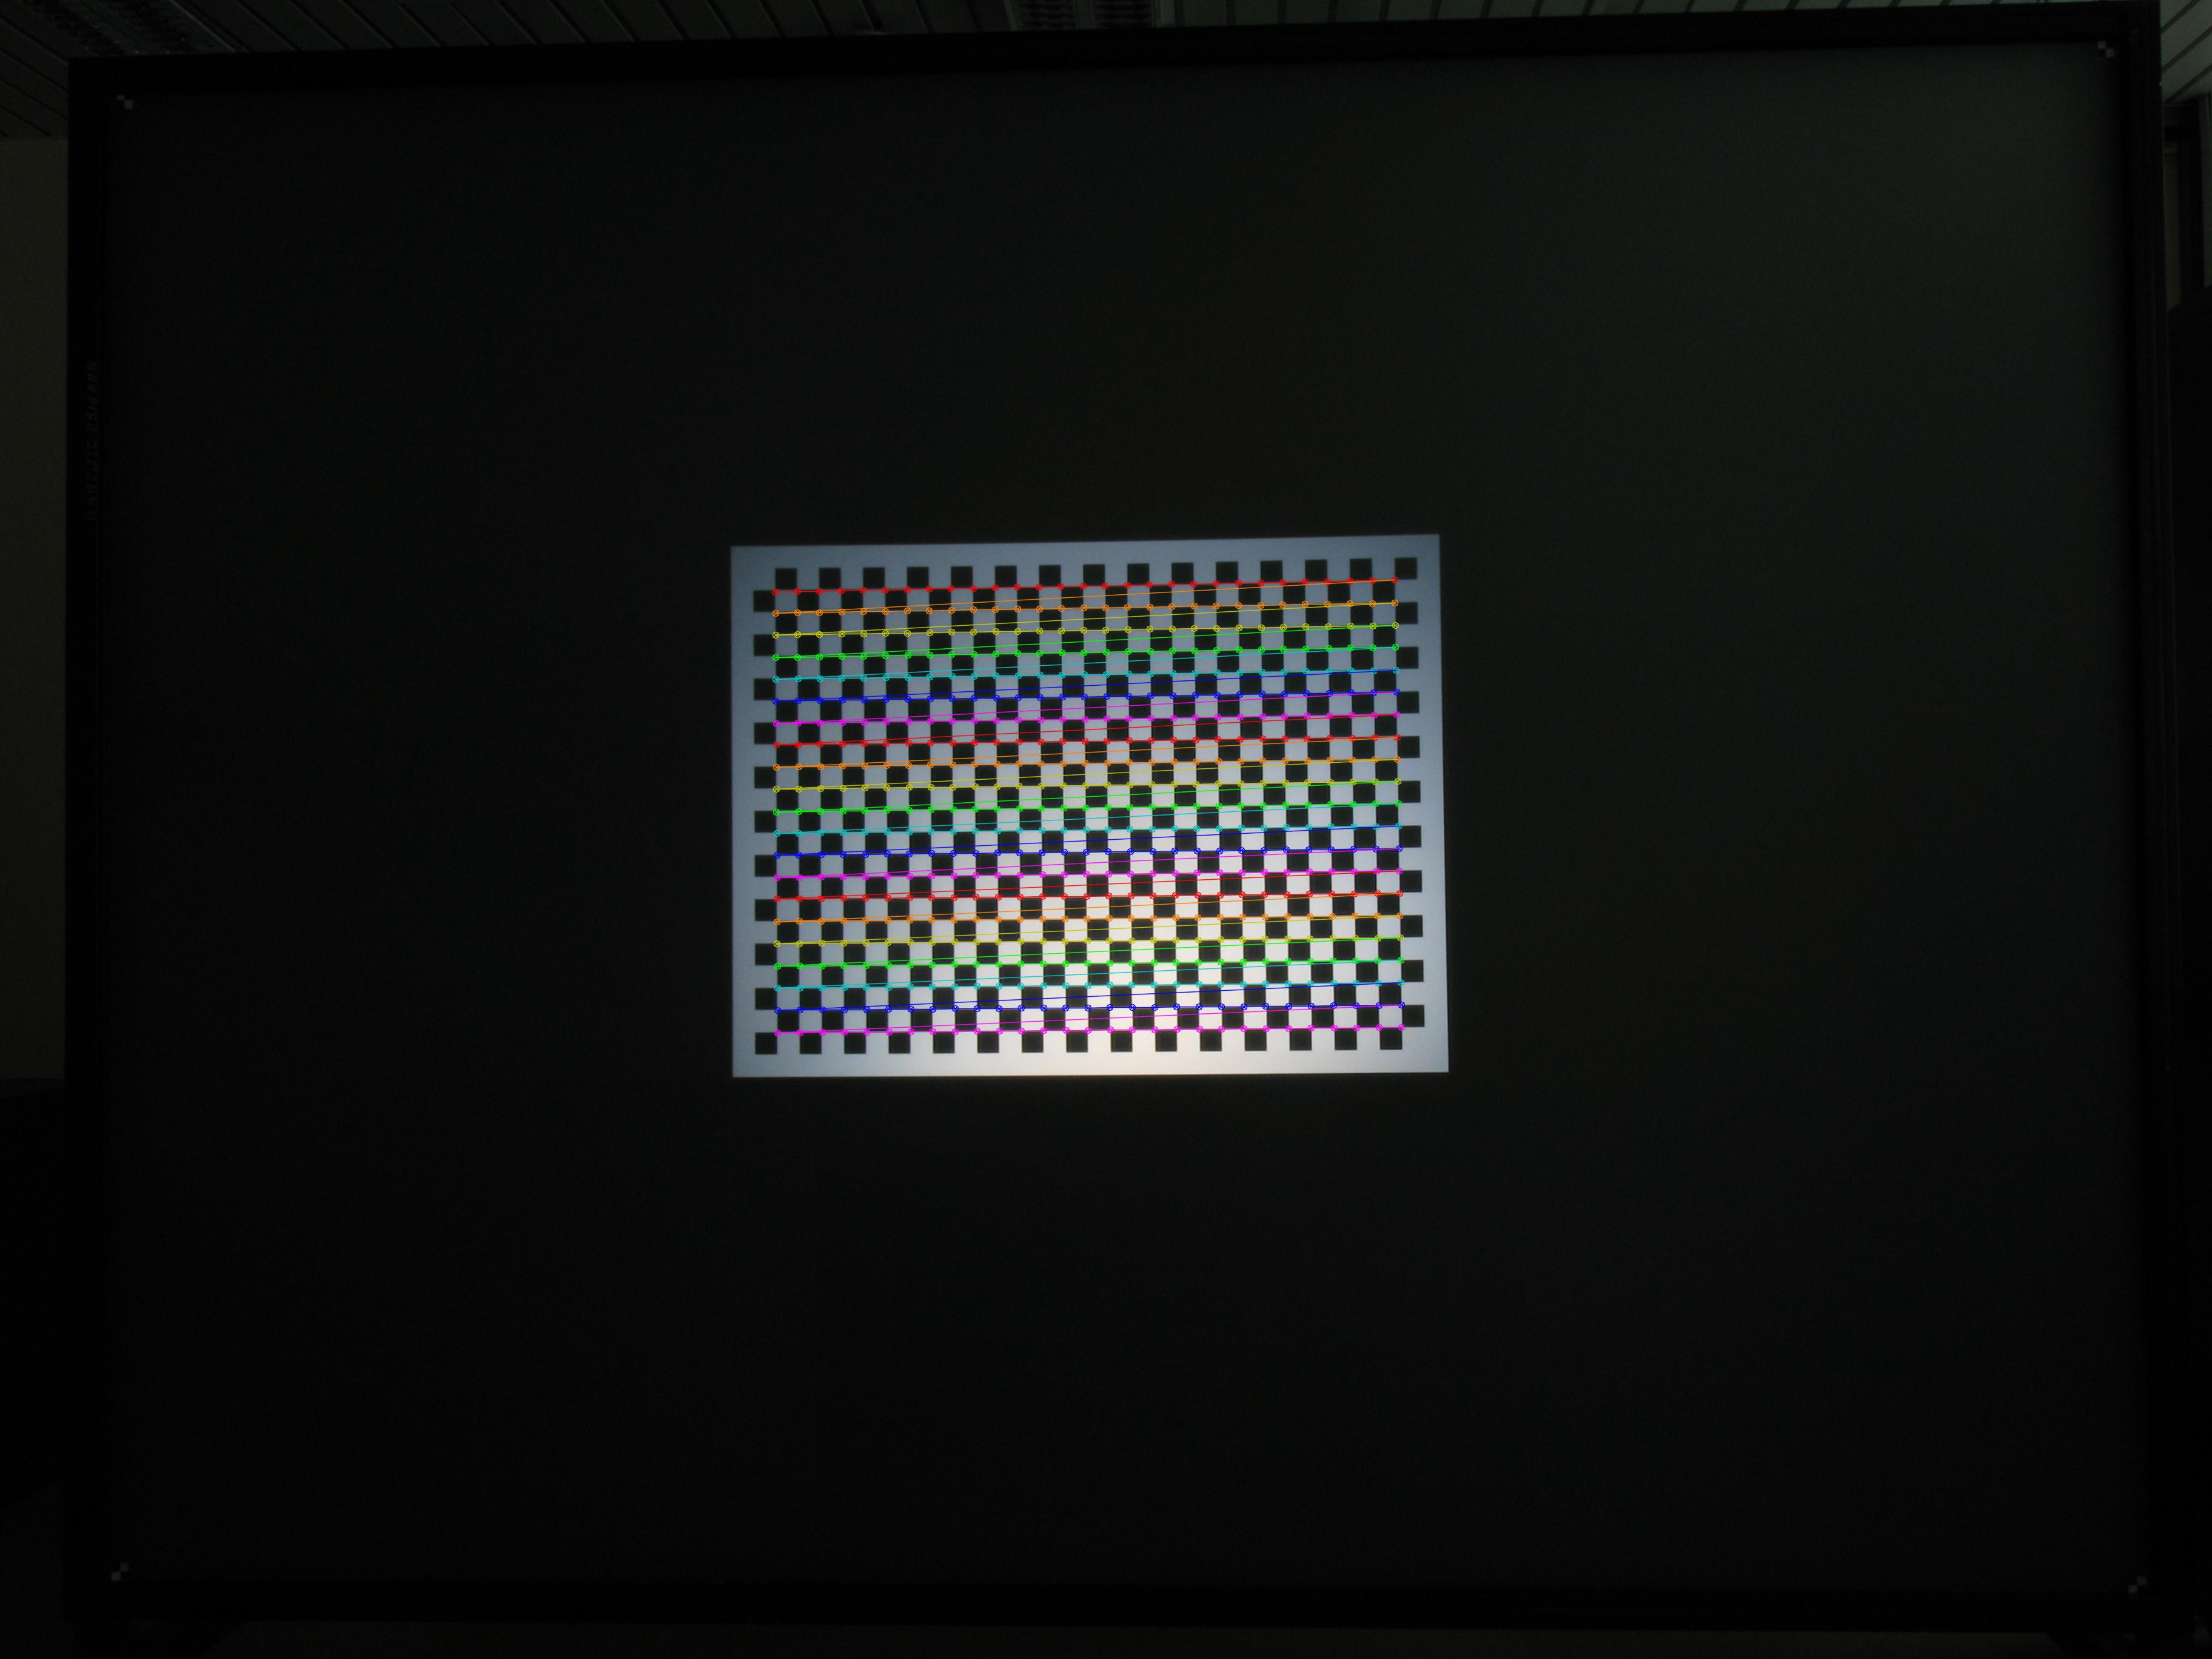
\includegraphics[width=6cm, height=4cm]{figures/detected_corners.jpg}} \\
\end{tabular}
\end{tabularx}
\end{figure}

\end{frame}

%//////////////////////////////////////////////////////////////////////////////////////////////////////////////////////////////////

\begin{frame}
\frametitle{Algorithm(contd.): Remove perspective distortion}
\framesubtitle{Compute \textit{local} bounding boxes}
Normalized pair of $(coordinate_{\textit{original image}}, coordinate_{\textit{detected}})$ for each checkerboard corner gives the \textit{\hyperlink{concept}{distortion}} information.
\begin{figure}
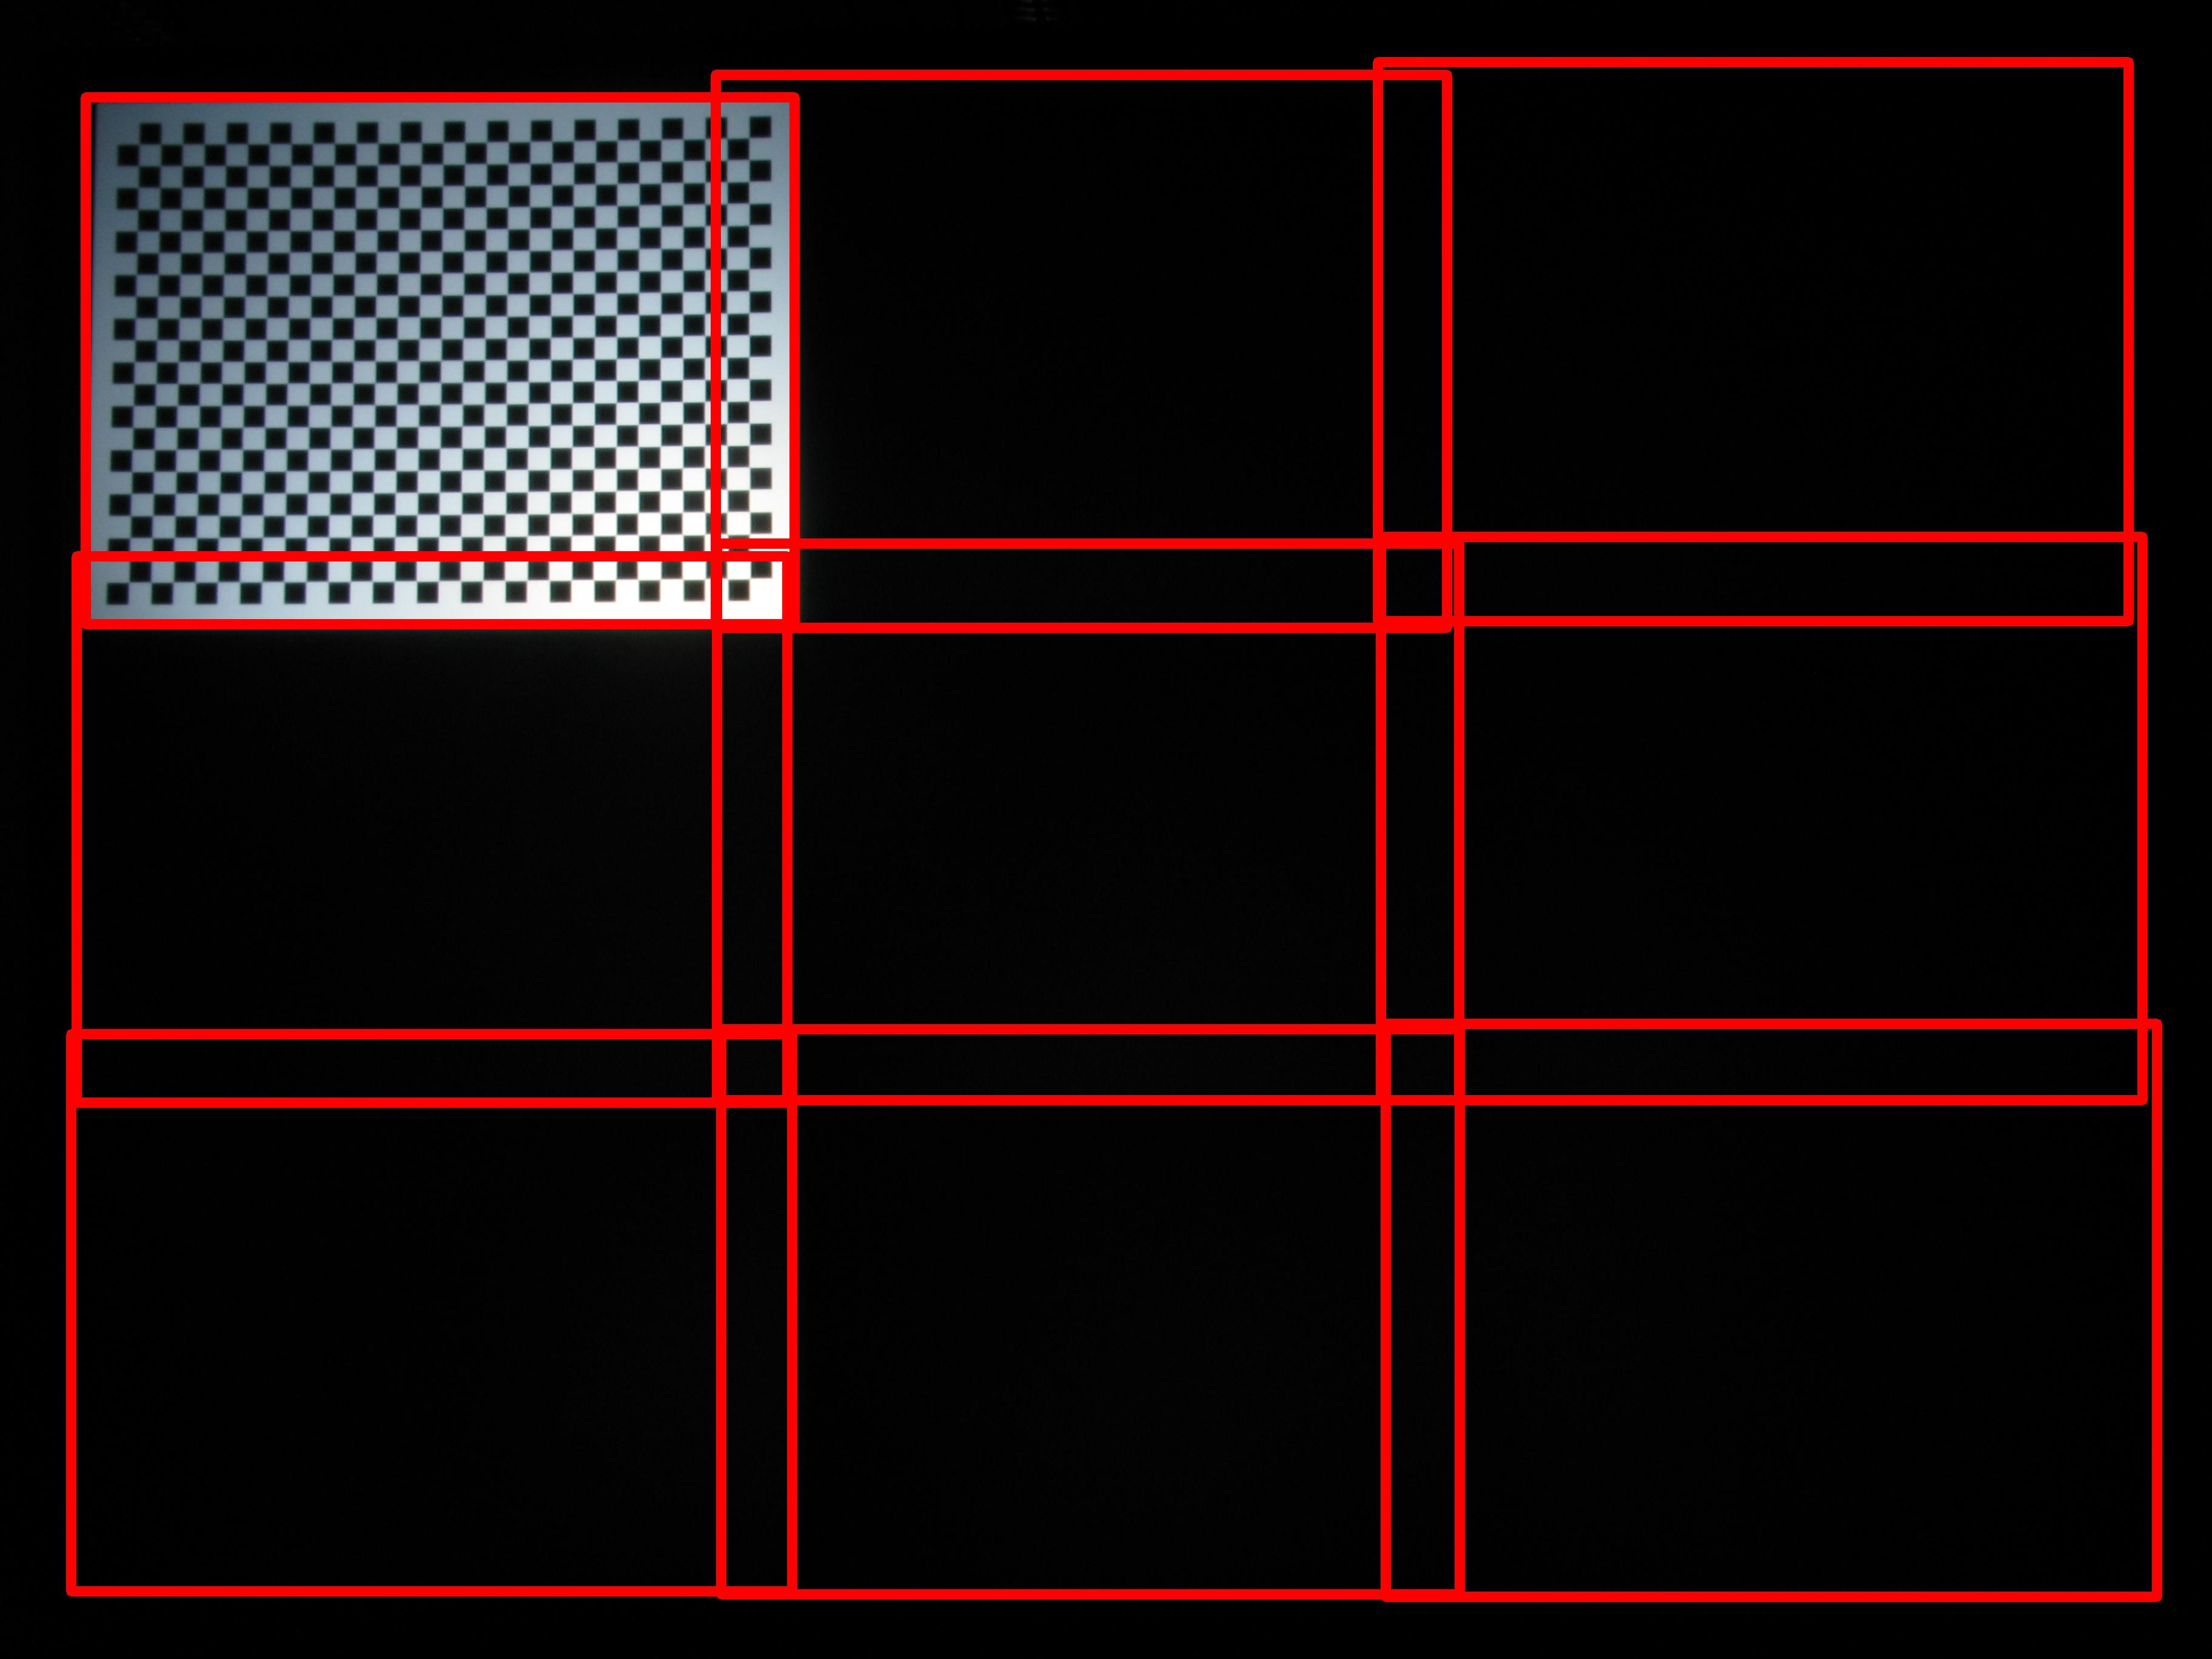
\includegraphics[width=6cm,height=4cm]{figures/all_bboxes.jpg}
\caption{Boxes bounding the projection region of each projector}
\end{figure}

\end{frame}

%//////////////////////////////////////////////////////////////////////////////////////////////////////////////////////////////////

\begin{frame}
\frametitle{Algorithm(contd.): Geometric continuity}
\framesubtitle{Compute \textit{global} bounding box}
\begin{itemize}
\item Addressing all local bounding boxes wrt. a common coordinate system. 
\item Global bounding box represents the original image to projected on the screen.
\item Helps in computing share of each projector in the original image.
\end{itemize}

\begin{figure}
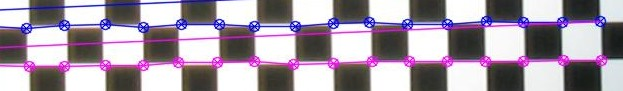
\includegraphics[width=6cm,height=4cm]{figures/test.jpg}
\end{figure}
\end{frame}

%//////////////////////////////////////////////////////////////////////////////////////////////////////////////////////////////////

\begin{frame}
\frametitle{Algorithm(contd.): Seamlessness}
\framesubtitle{Compute alpha map}
\begin{enumerate}
\item Compute \hyperlink{concept}{region of overlap} between adjacent projectors.
\item Attenuate image intensity of each overlapping projector.
\end{enumerate}

\begin{figure}
\centering
\begin{tabularx}{\linewidth}{@{}cXX@{}}
\begin{tabular}{c c}
\hspace{0.5cm}\subfloat[Projection region]{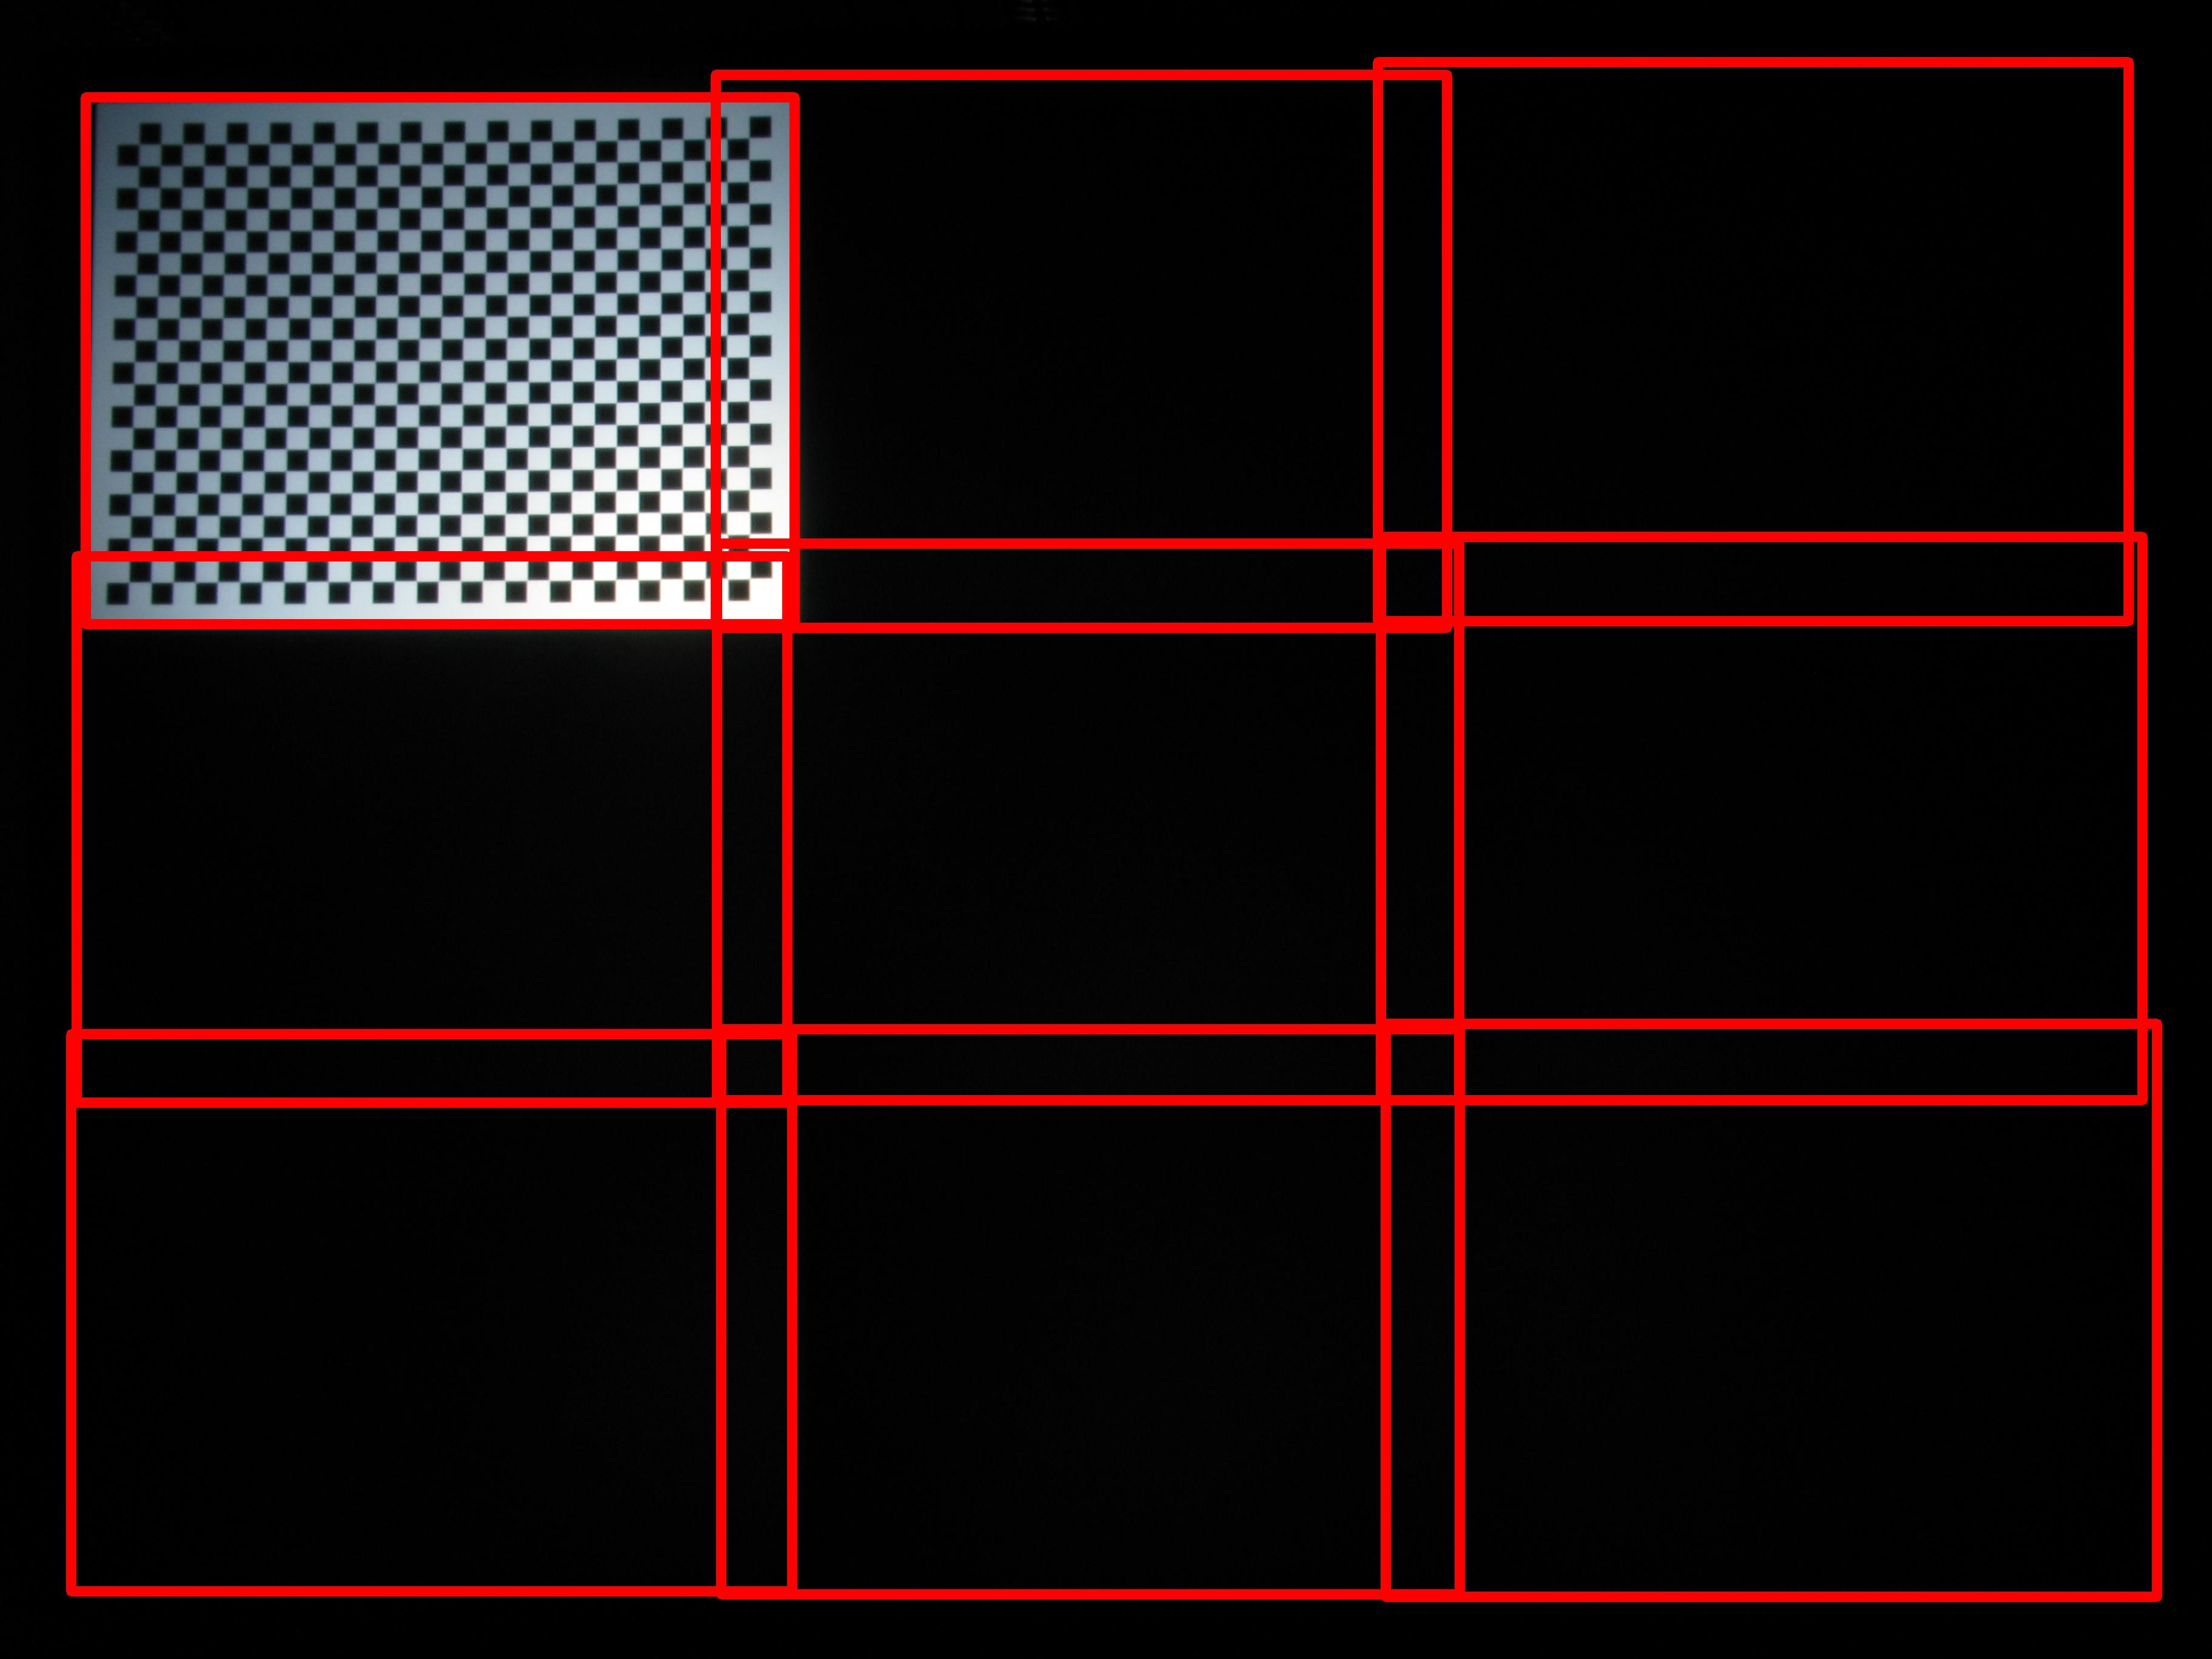
\includegraphics[width=4.5cm,height=3cm]{figures/all_bboxes.jpg}} &
\subfloat[Corresponding attenuation map]{
\includegraphics[width=4.5cm,height=3cm]{figures/alpha_map_6.jpg}} \\
\end{tabular}
\end{tabularx}
\end{figure}

\end{frame}

%//////////////////////////////////////////////////////////////////////////////////////////////////////////////////////////////////

\begin{frame}

\frametitle{Contributions}
\underline{Corrected detected corners using line fitting}:
\begin{itemize}
\item Utilized the fact that collinearity under perspective projection is preserved.
\item Fitted line on detected corners and corrected the detected coordinates using intersection of fitted lines.
\item It resulted in more uniform texture mapping.
\end{itemize}

\begin{figure}
\centering
\begin{tabularx}{\linewidth}{@{}cXX@{}}
\begin{tabular}{c c}
\hspace{0.5cm}\subfloat[Without line fitting]{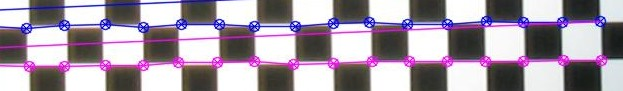
\includegraphics[width=4.5cm,height=1.0cm]{figures/test1.jpg}} & 
\subfloat[With line fitting]{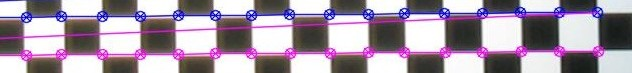
\includegraphics[width=4.5cm,height=1.0cm]{figures/test2.jpg}} \\
\end{tabular}
\end{tabularx}
\end{figure}

\end{frame}

%//////////////////////////////////////////////////////////////////////////////////////////////////////////////////////////////////

\begin{frame}{Contributions(contd.)}

\underline{Used \hyperlink{crossrat}{Cross-ratio invariant} to recover full projection region}:

\begin{itemize}
\item It is a perspective projection invariant.
\item Relates 4 collinear points:
$CR_p=\frac{|AC|_c*|BD|_c}{|BC|_c*|AD|_c}$
\end{itemize}

\begin{figure}
\centering
\begin{tabularx}{\linewidth}{@{}cXX@{}}
\begin{tabular}{c c}
\subfloat[Applying cross ratio invariant]{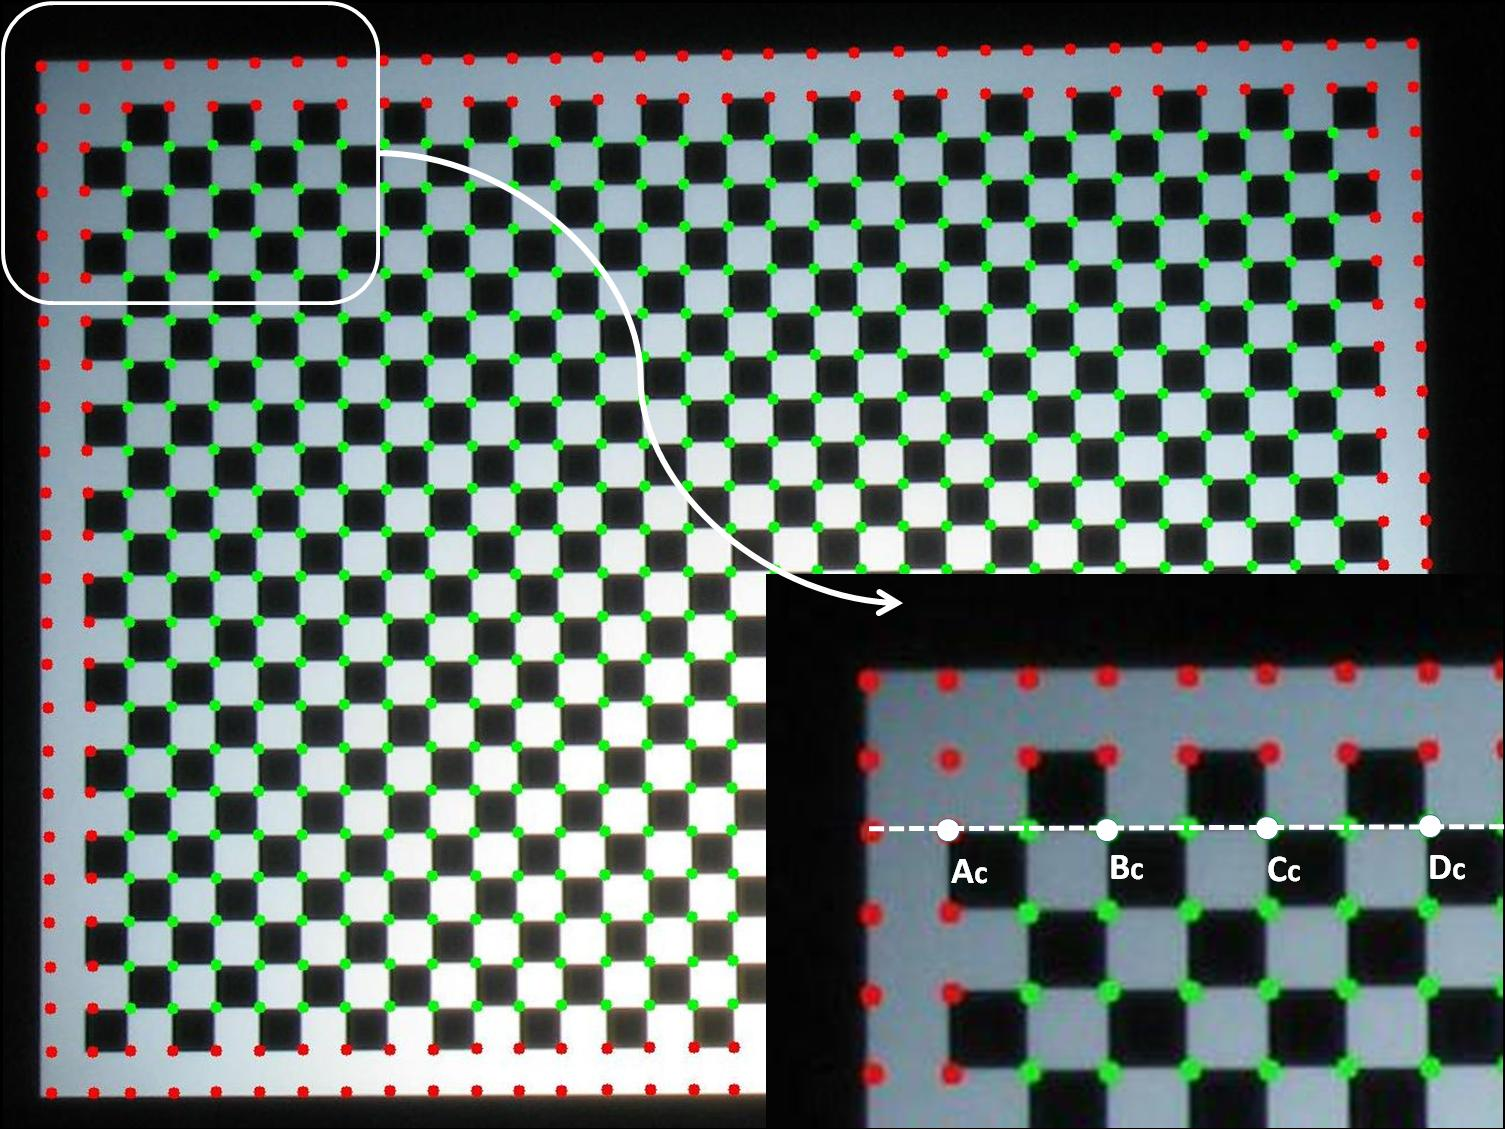
\includegraphics[width=5.0cm,height=4.0cm]{figures/cross_rat_img.jpg}} &
\subfloat[green: without cross ratio, blue: with cross ratio invariant]{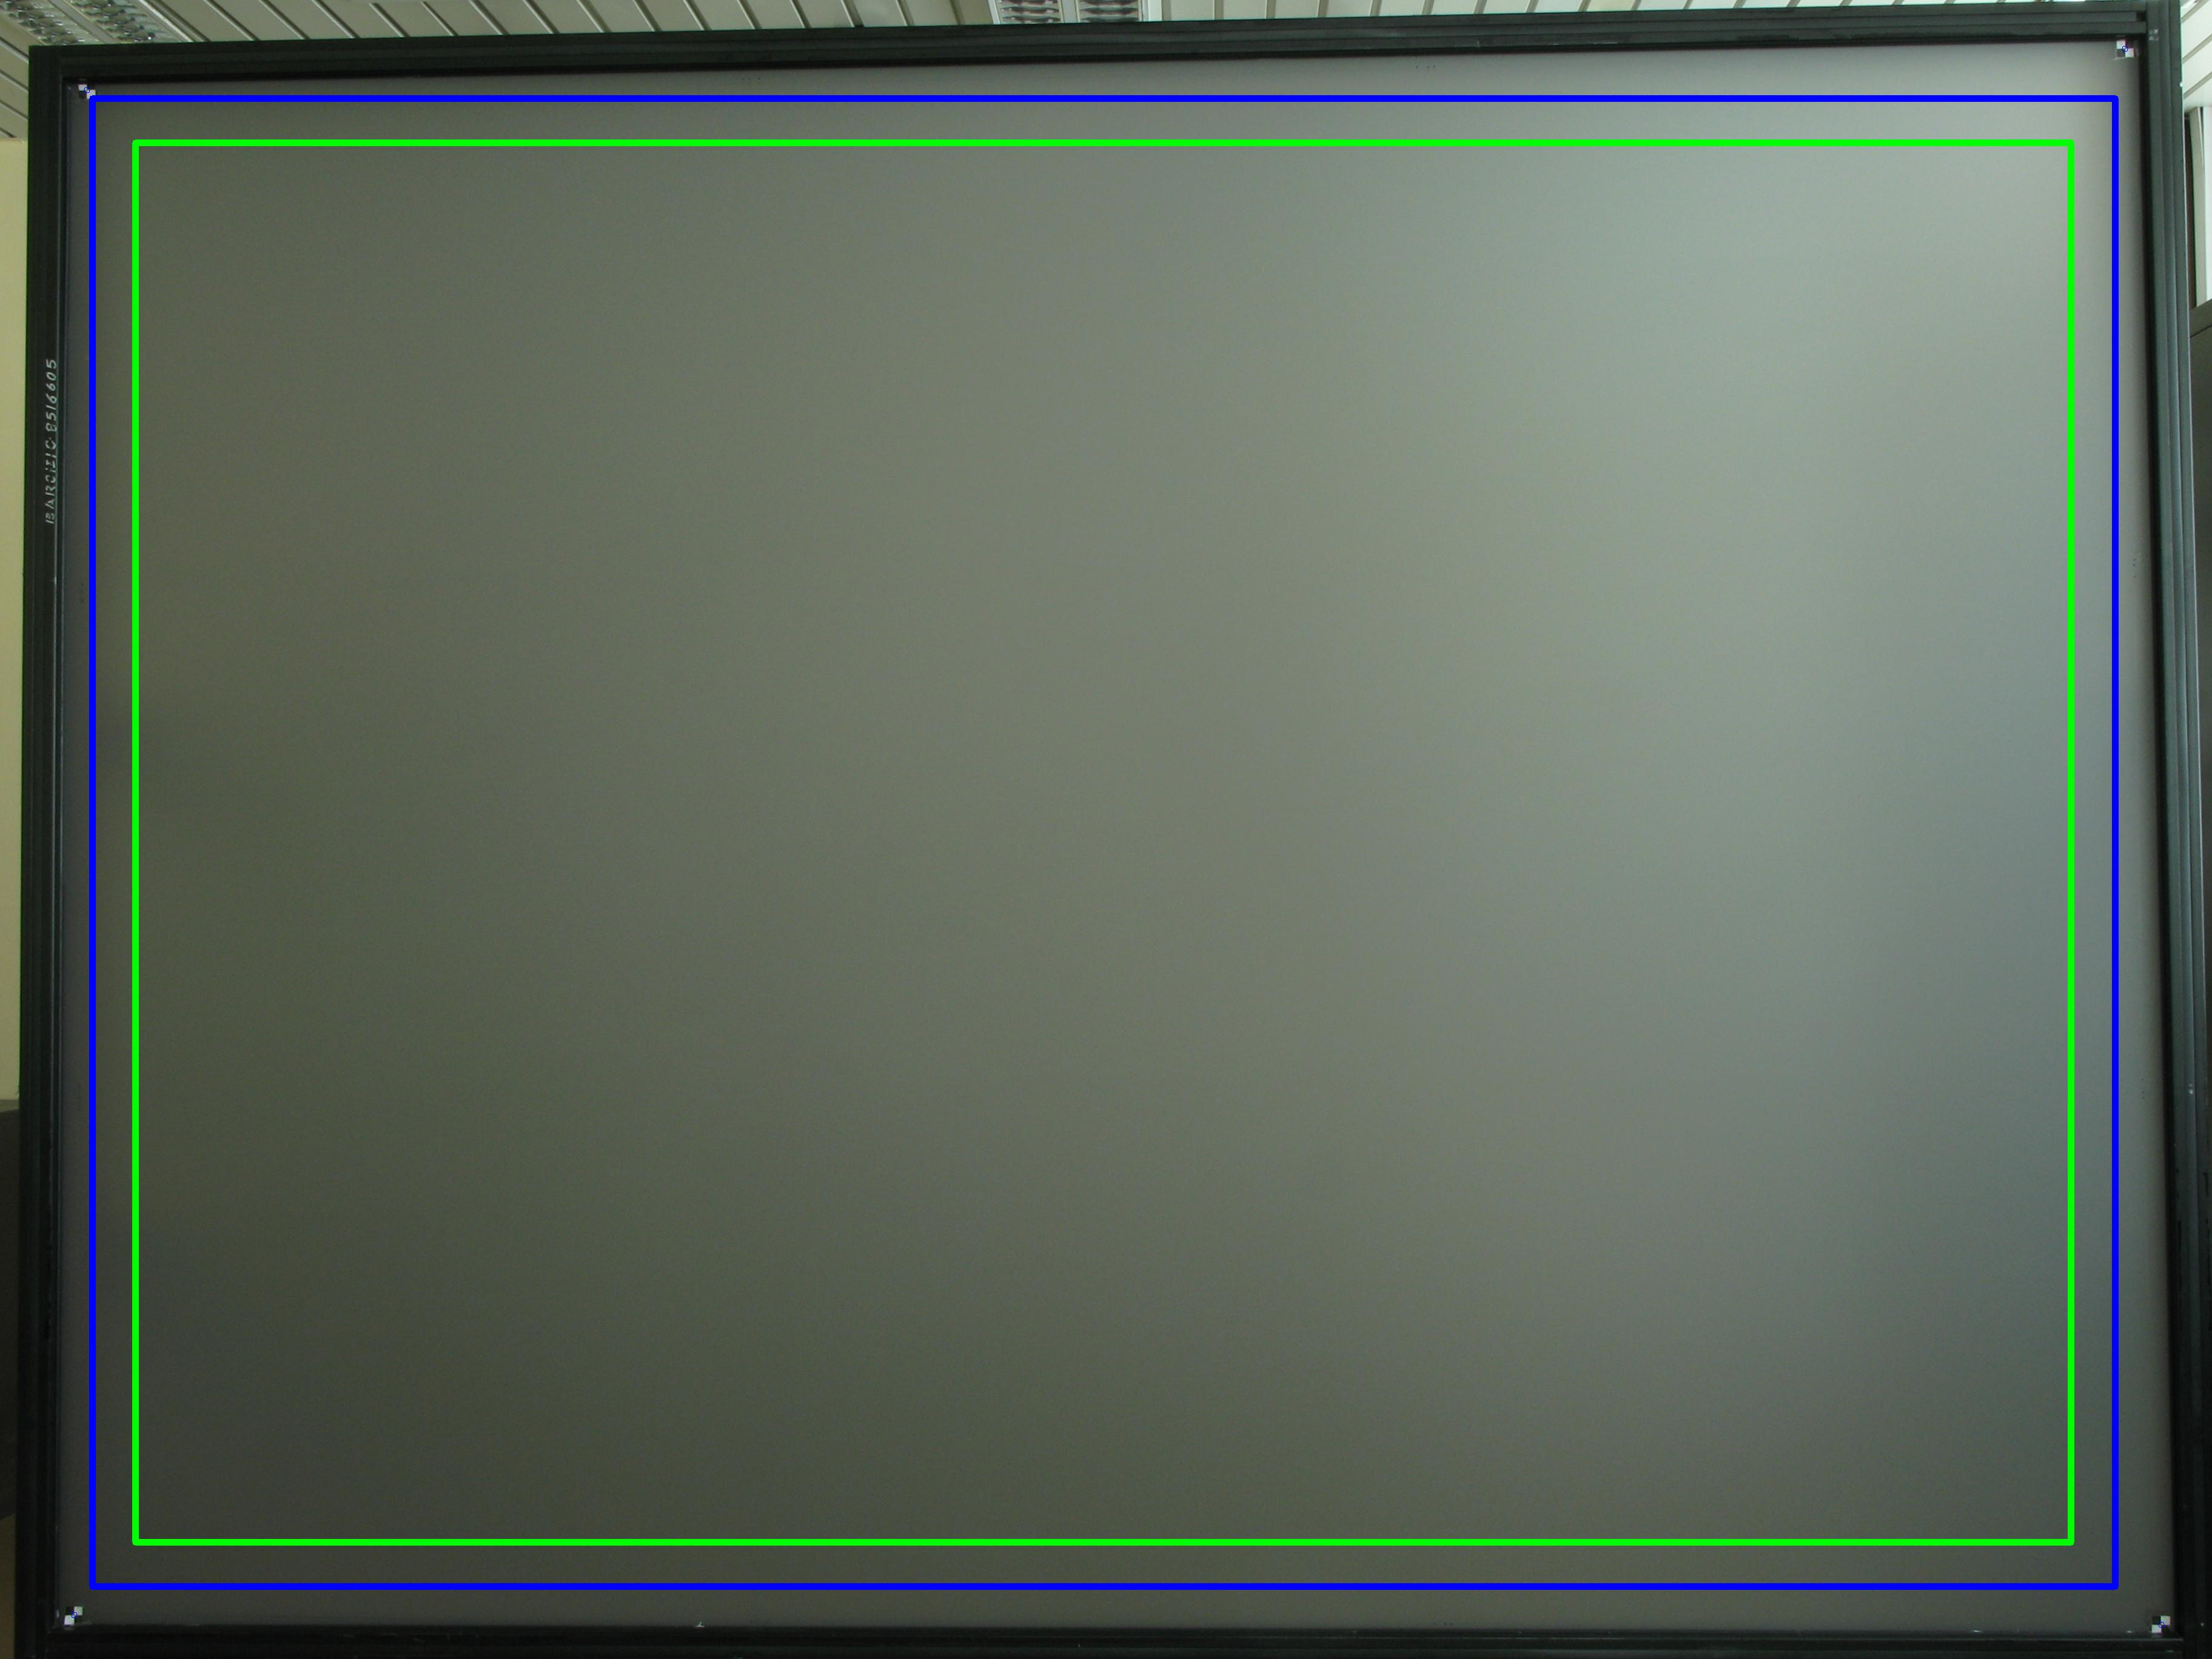
\includegraphics[width=5.0cm,height=4.0cm]{figures/crossratio_vs_noncrossratio.jpg}} \\
\end{tabular}
\end{tabularx}
\end{figure}


\end{frame}

%//////////////////////////////////////////////////////////////////////////////////////////////////////////////////////////////////

\begin{frame}
\frametitle{Results\textsuperscript{\hyperlink{sysconfg}{*}}}
\begin{itemize}
\item Alignment procedure completes in 3-4 minutes as opposed to $\sim30$ mins. consumed in our earlier alignment approaches.
\item Average misalignment between the grid lines projected at junction between neighbouring projectors was around $\sim1.0mm$ on a grid size of $\sim14$mm.
\begin{figure}
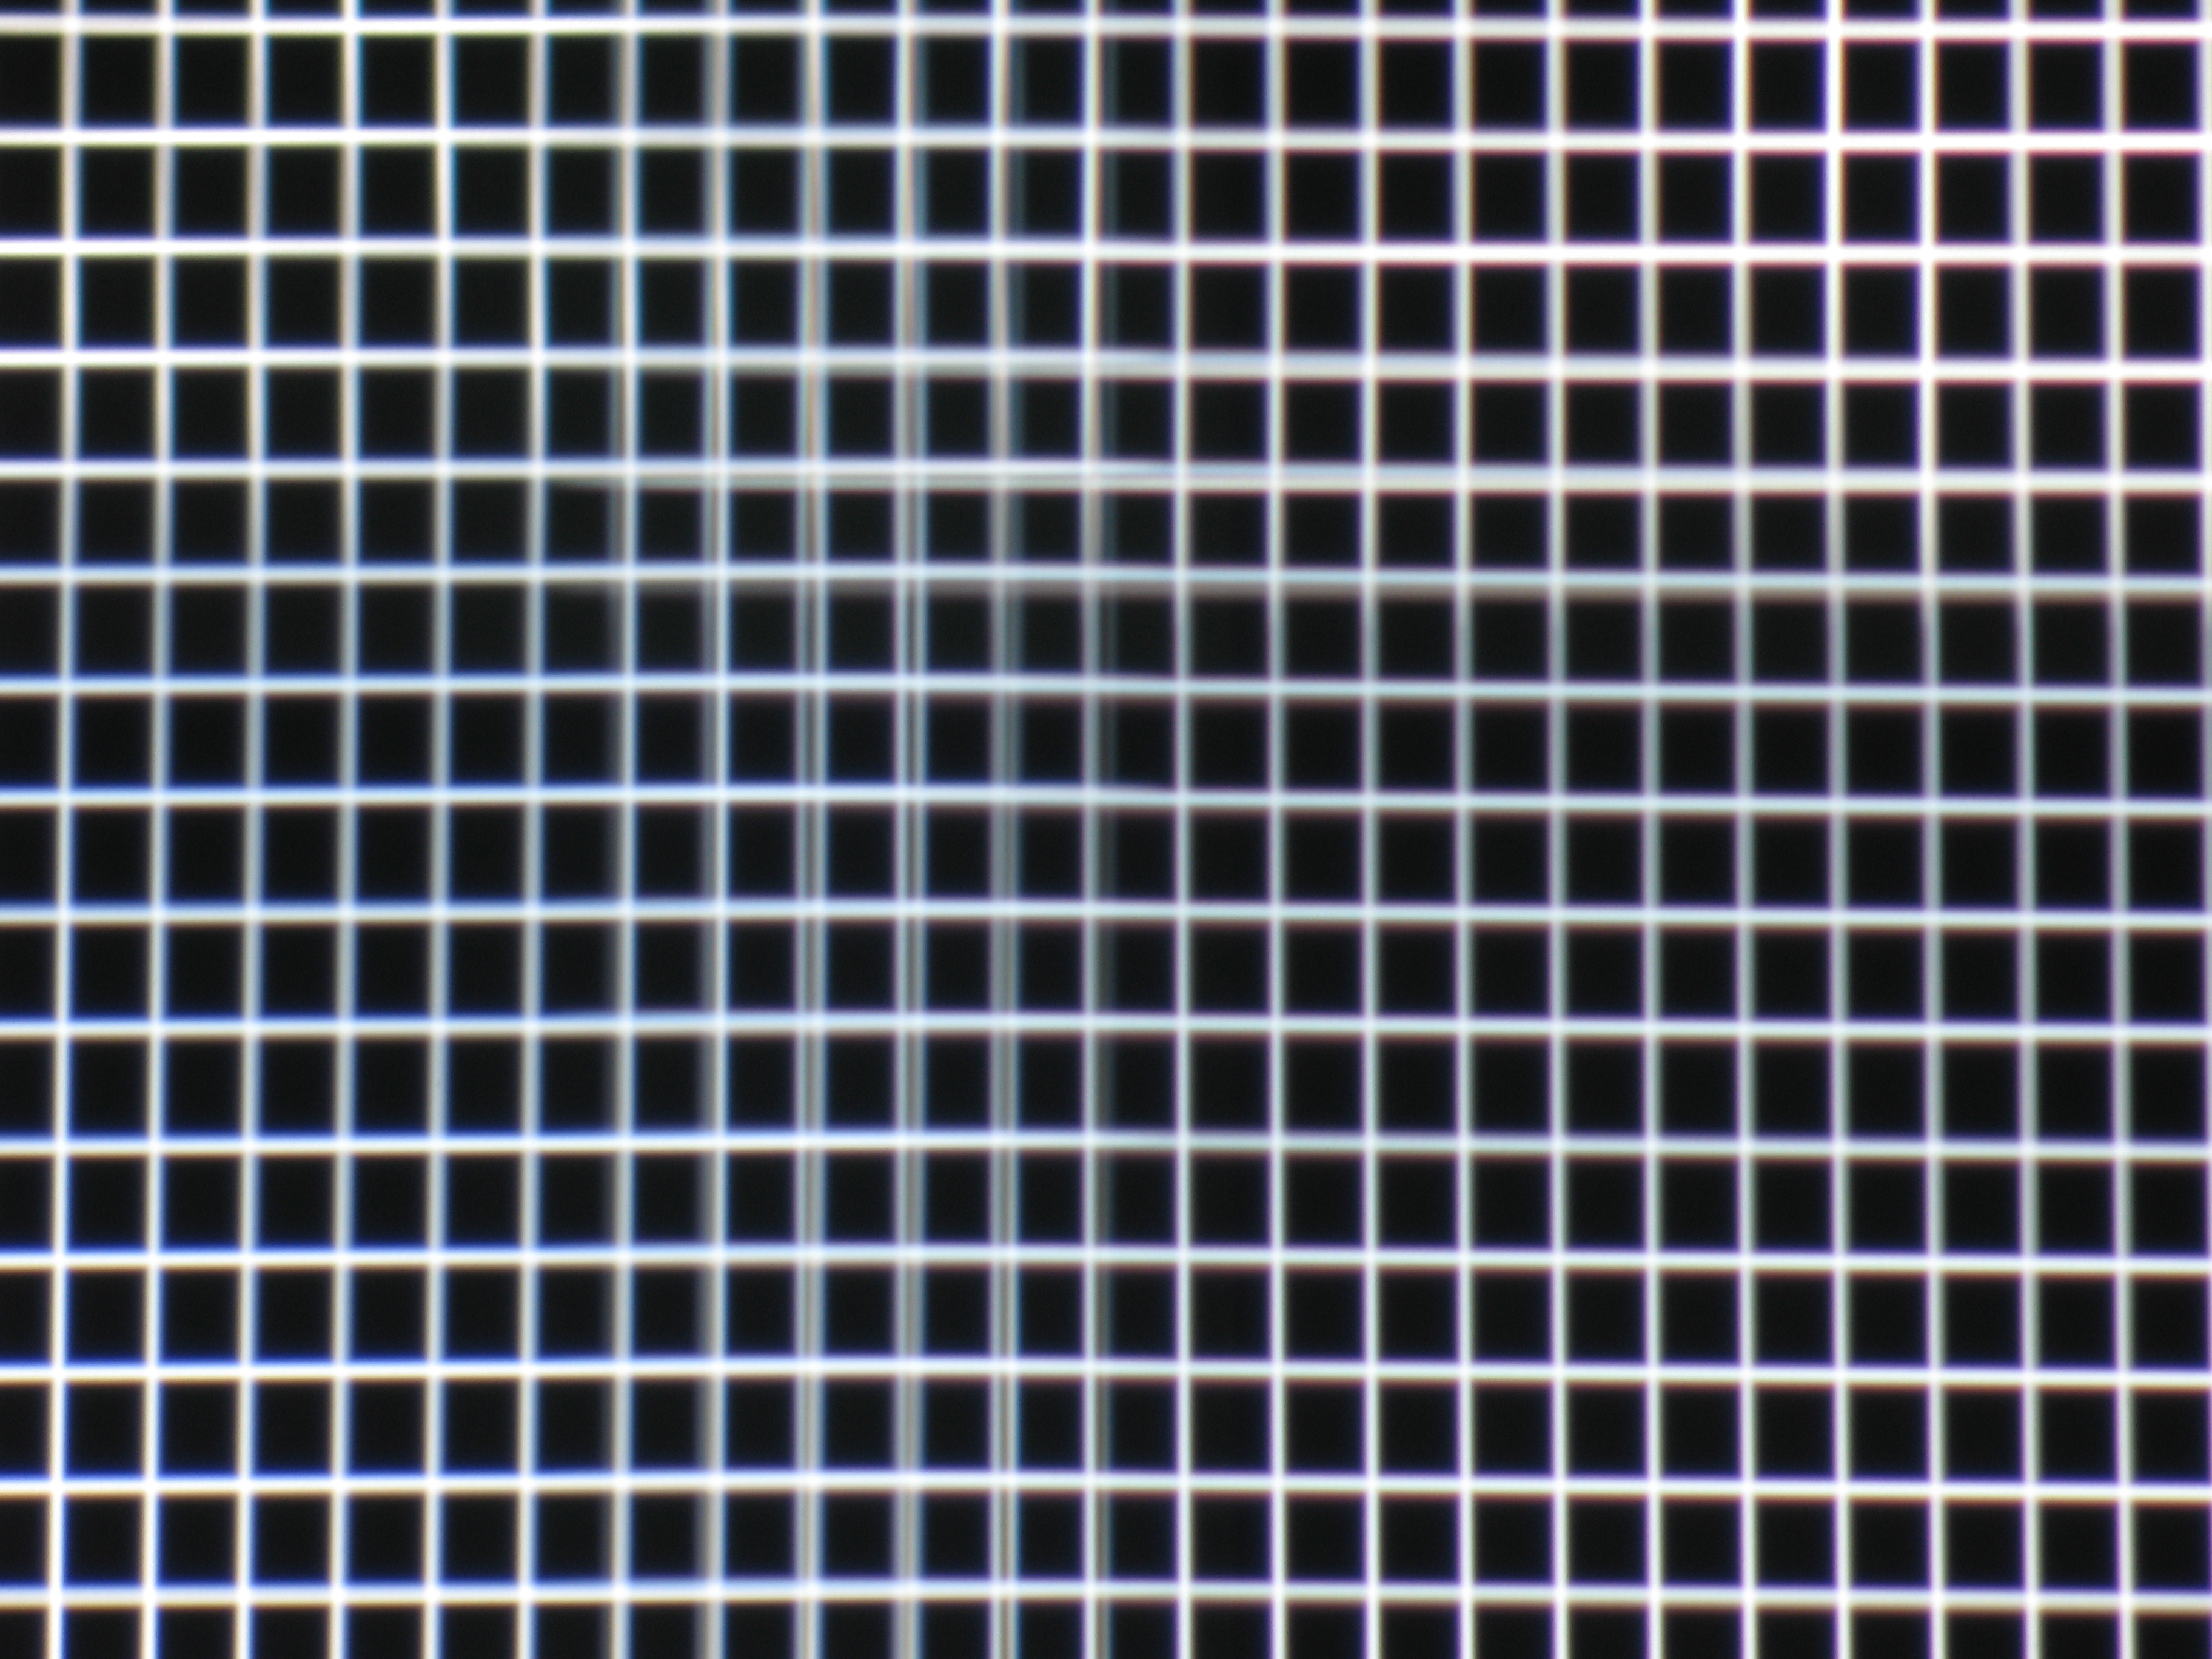
\includegraphics[width=6cm, height=4cm]{figures/grid.jpg}
\end{figure}
\end{itemize}
\end{frame}


\begin{frame}{Results(contd.)}
\begin{itemize}
\item Recovered $\sim10$\% more projection region using cross-ratio invariant.
\item Junctions between projectors are more imperceptible using cross ratio invariant.
\begin{figure}
\centering
\begin{tabularx}{\linewidth}{@{}cXX@{}}
\begin{tabular}{c c}
\hspace{0.5cm}\subfloat[Without cross ratio: seams more visible]{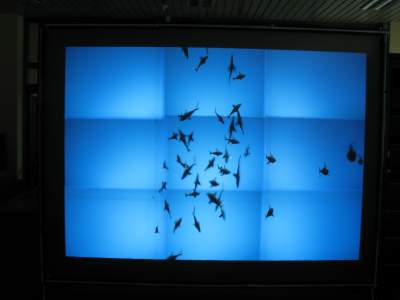
\includegraphics[width=4.0cm,height=3.0cm]{figures/without_cross_rat1.jpg}} &
\subfloat[With cross ratio: seams more imperceptible]{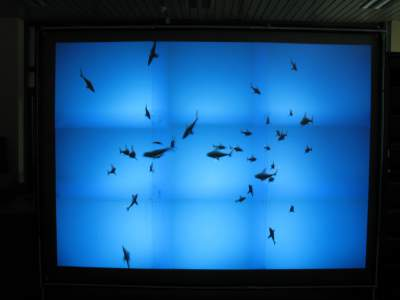
\includegraphics[width=4.0cm,height=3.0cm]{figures/with_cross_rat1.jpg}} \\
\end{tabular}
\end{tabularx}
\end{figure}

\item Resolution of the display is $\sim6.2$ Megapixels. 
\end{itemize}
\end{frame}

%//////////////////////////////////////////////////////////////////////////////////////////////////////////////////////////////////

\begin{frame}
\frametitle{Issues}
\begin{itemize}
\item Blending function which can provide \textit{completely} imperceptible seams in the overlapping regions is unknown. 
\item View dependant bright spot formation is still an \textit{open} problem.
\end{itemize}

\begin{figure}
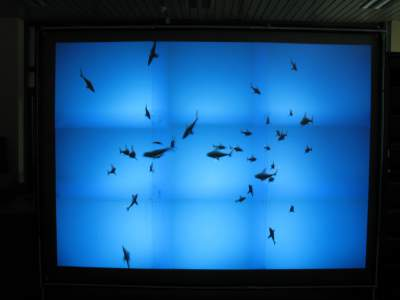
\includegraphics[width=6.0cm,height=4.0cm]{figures/with_cross_rat1.jpg}
\caption{Open issues}
\end{figure}
\end{frame}

%//////////////////////////////////////////////////////////////////////////////////////////////////////////////////////////////////

\begin{frame}{Some snapshots}

\begin{figure}
\centering
\begin{tabularx}{\linewidth}{@{}cXX@{}}
\begin{tabular}{c c}
\subfloat[]{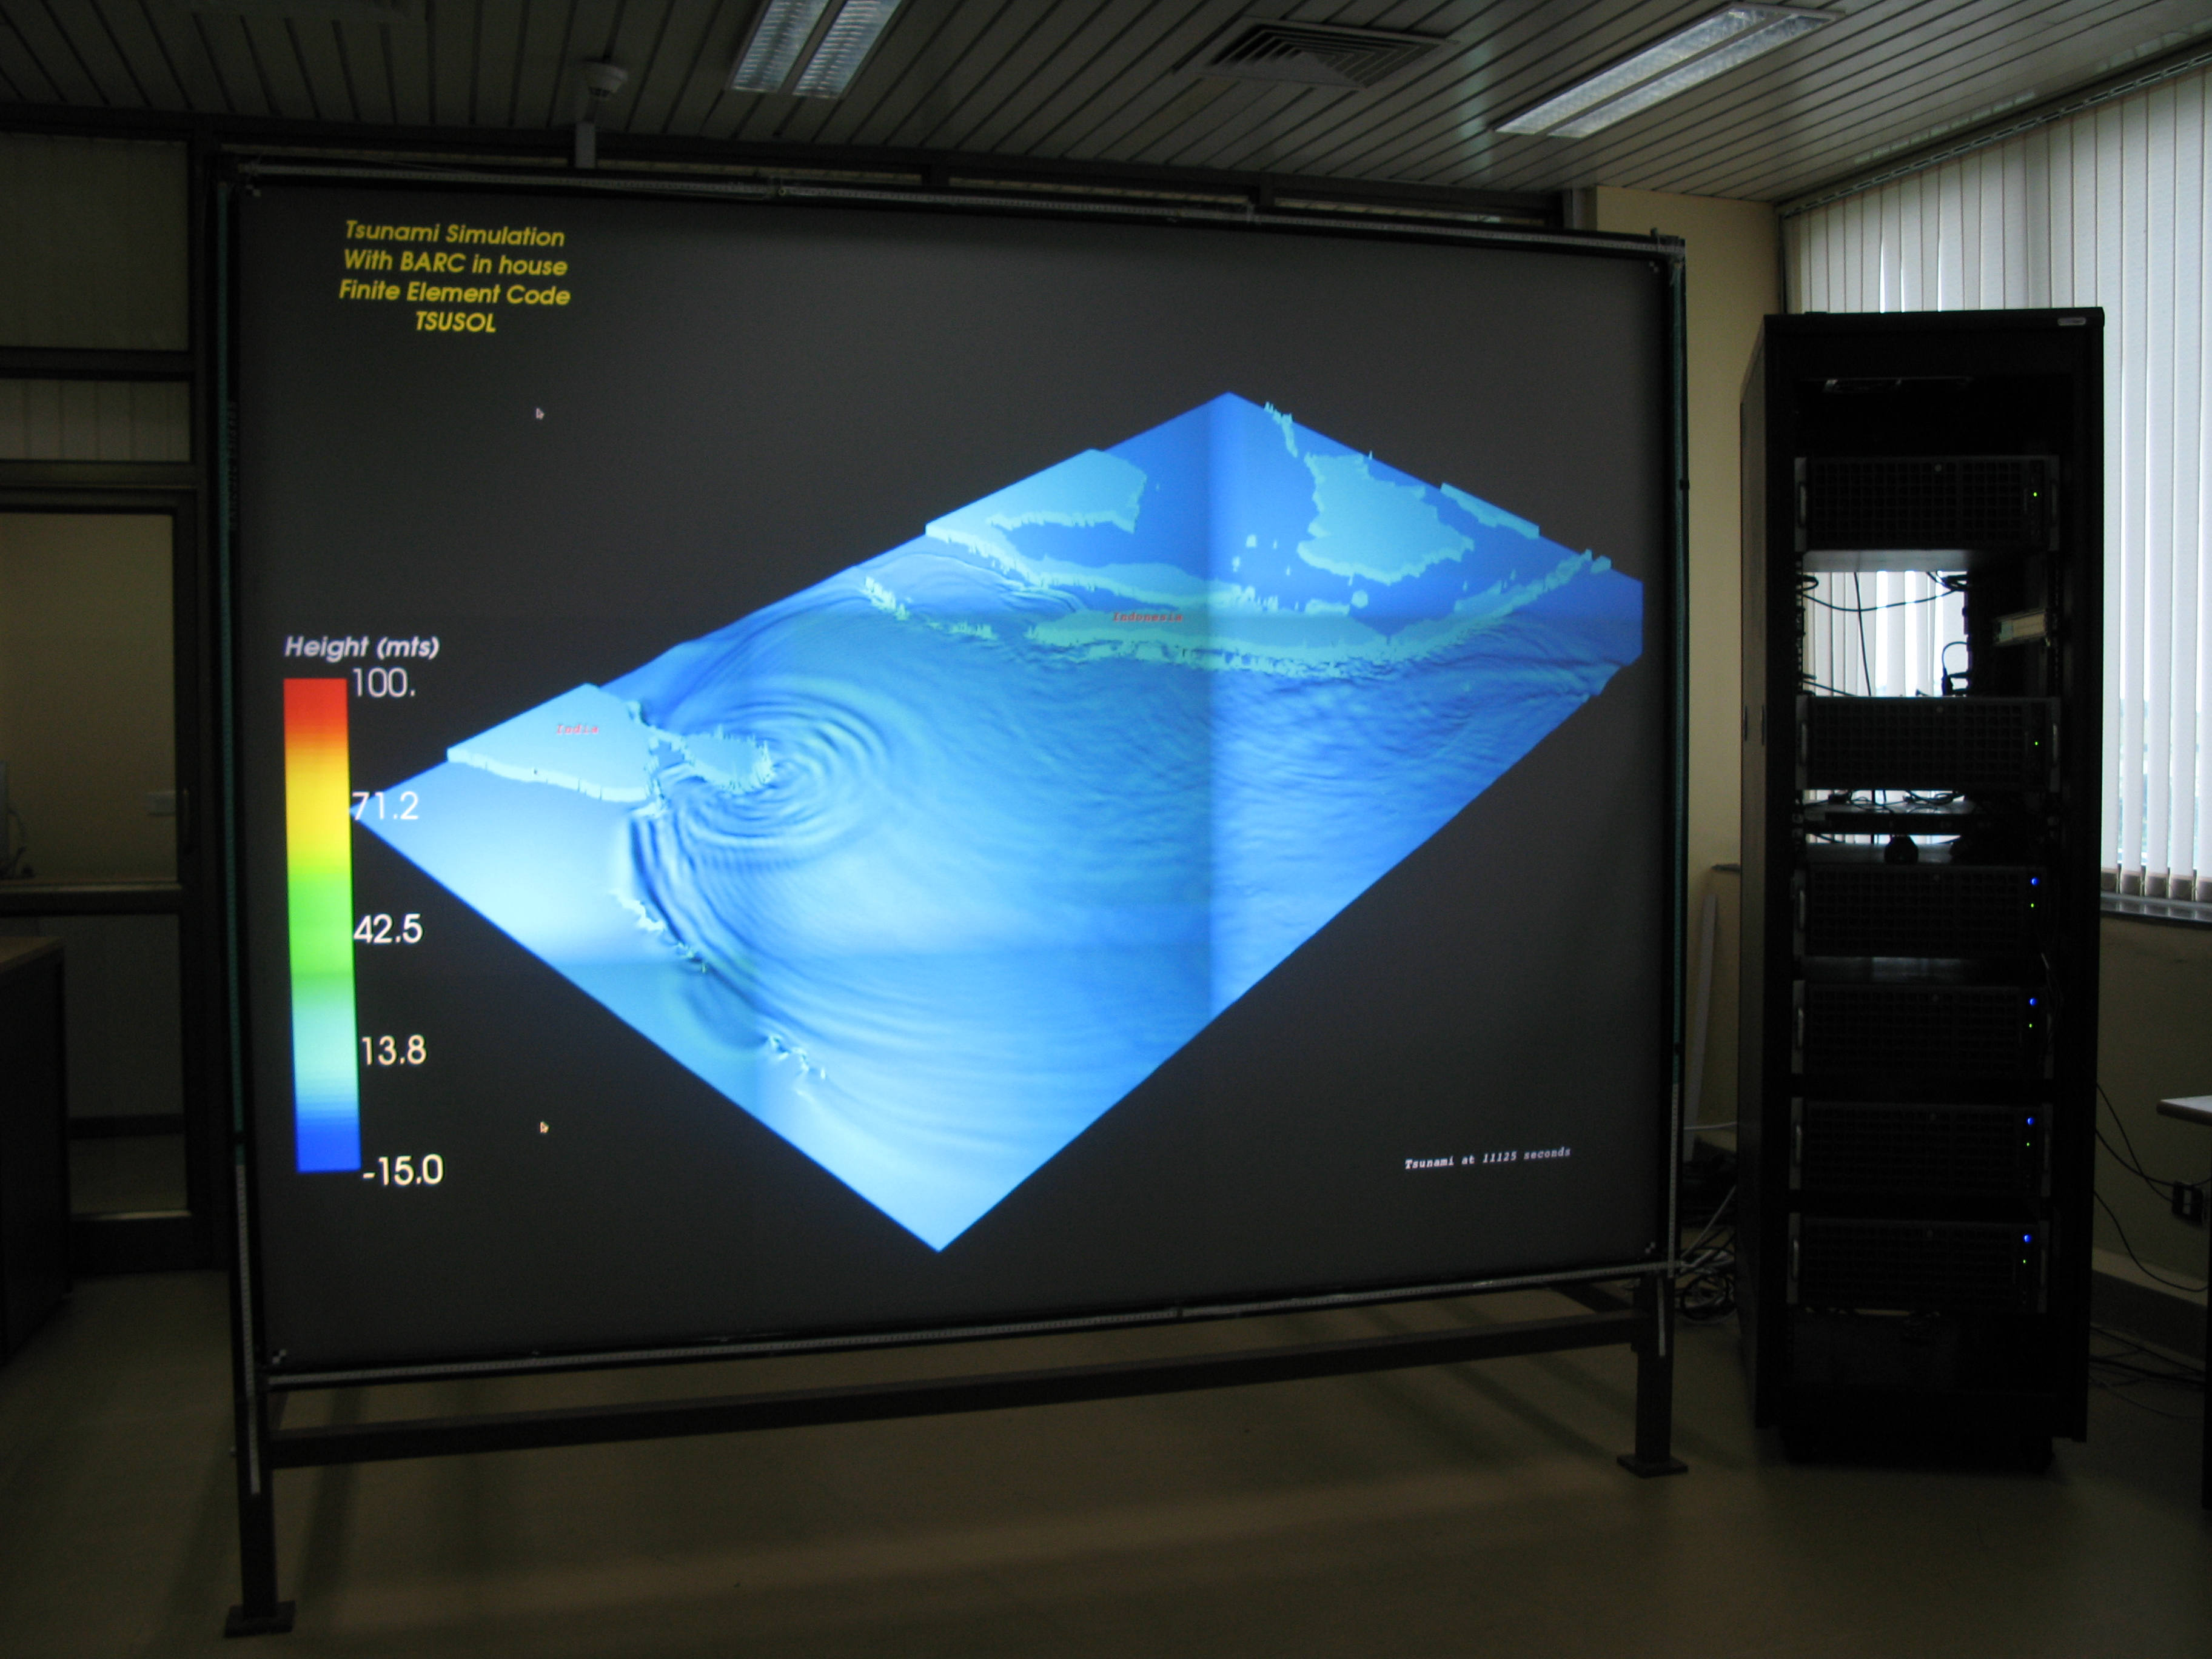
\includegraphics[width=5cm,height=3cm]{figures/1.JPG}} &
\subfloat[]{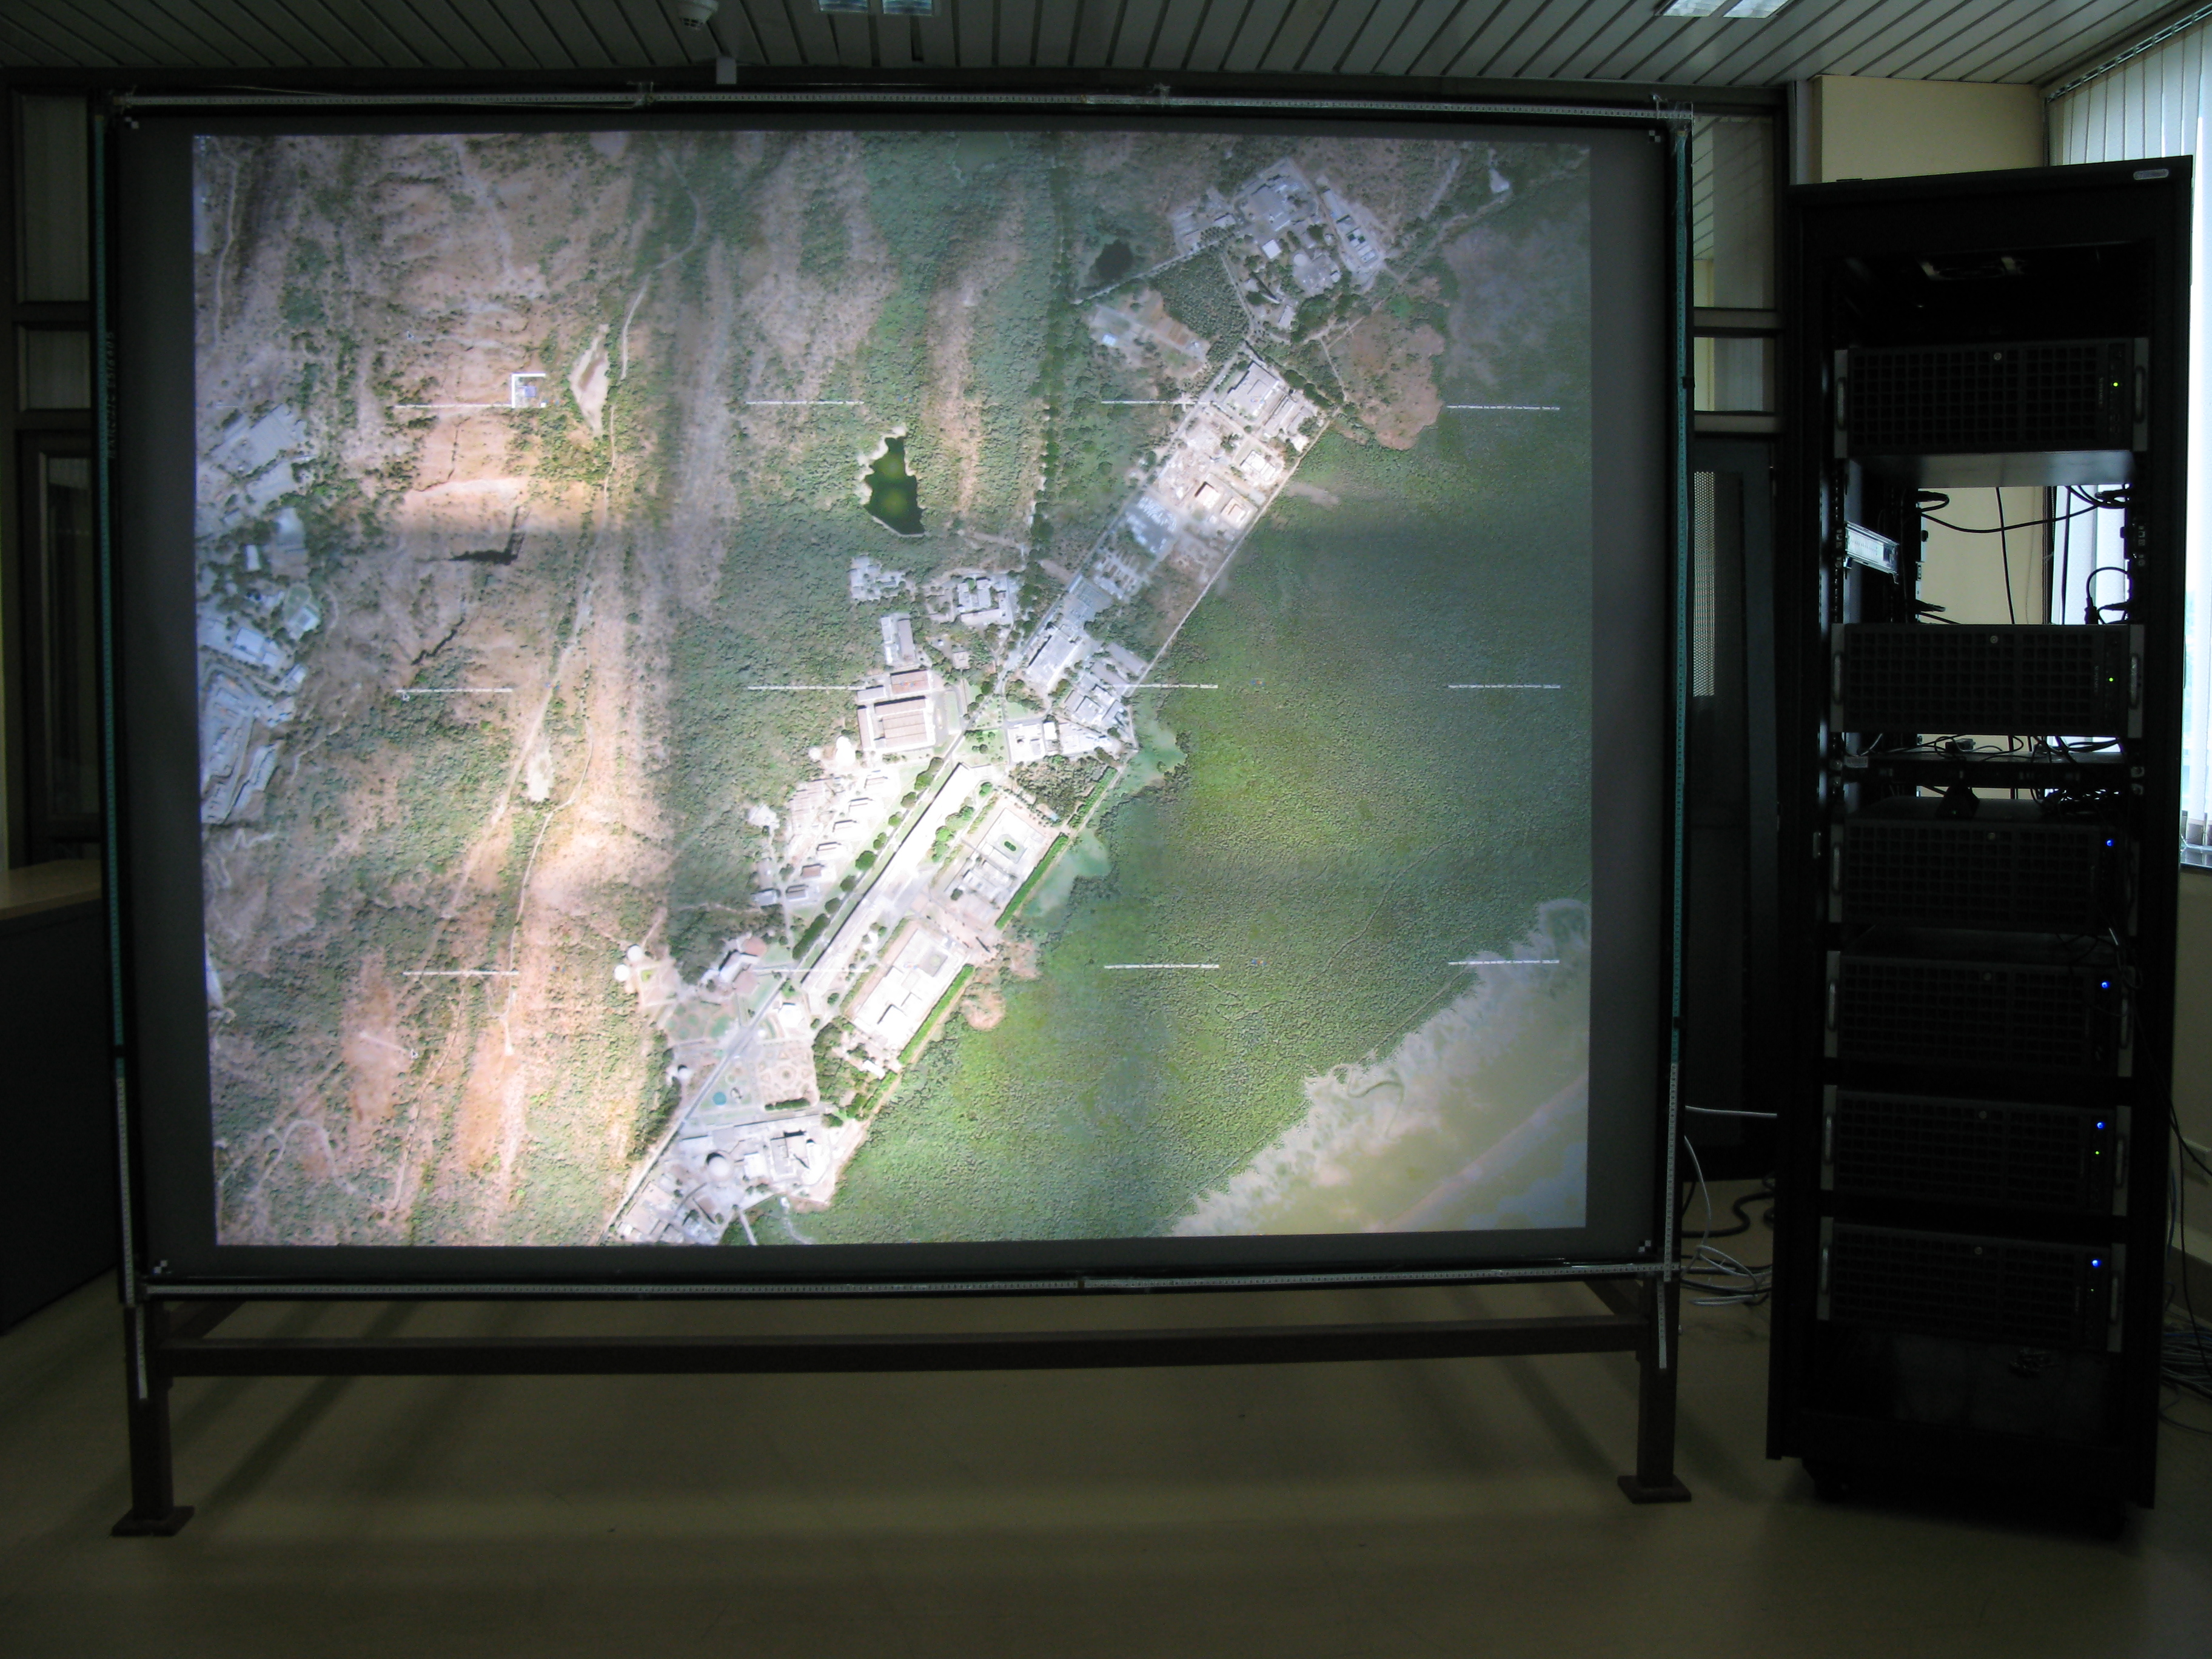
\includegraphics[width=5cm,height=3cm]{figures/2.JPG}} \\
\subfloat[]{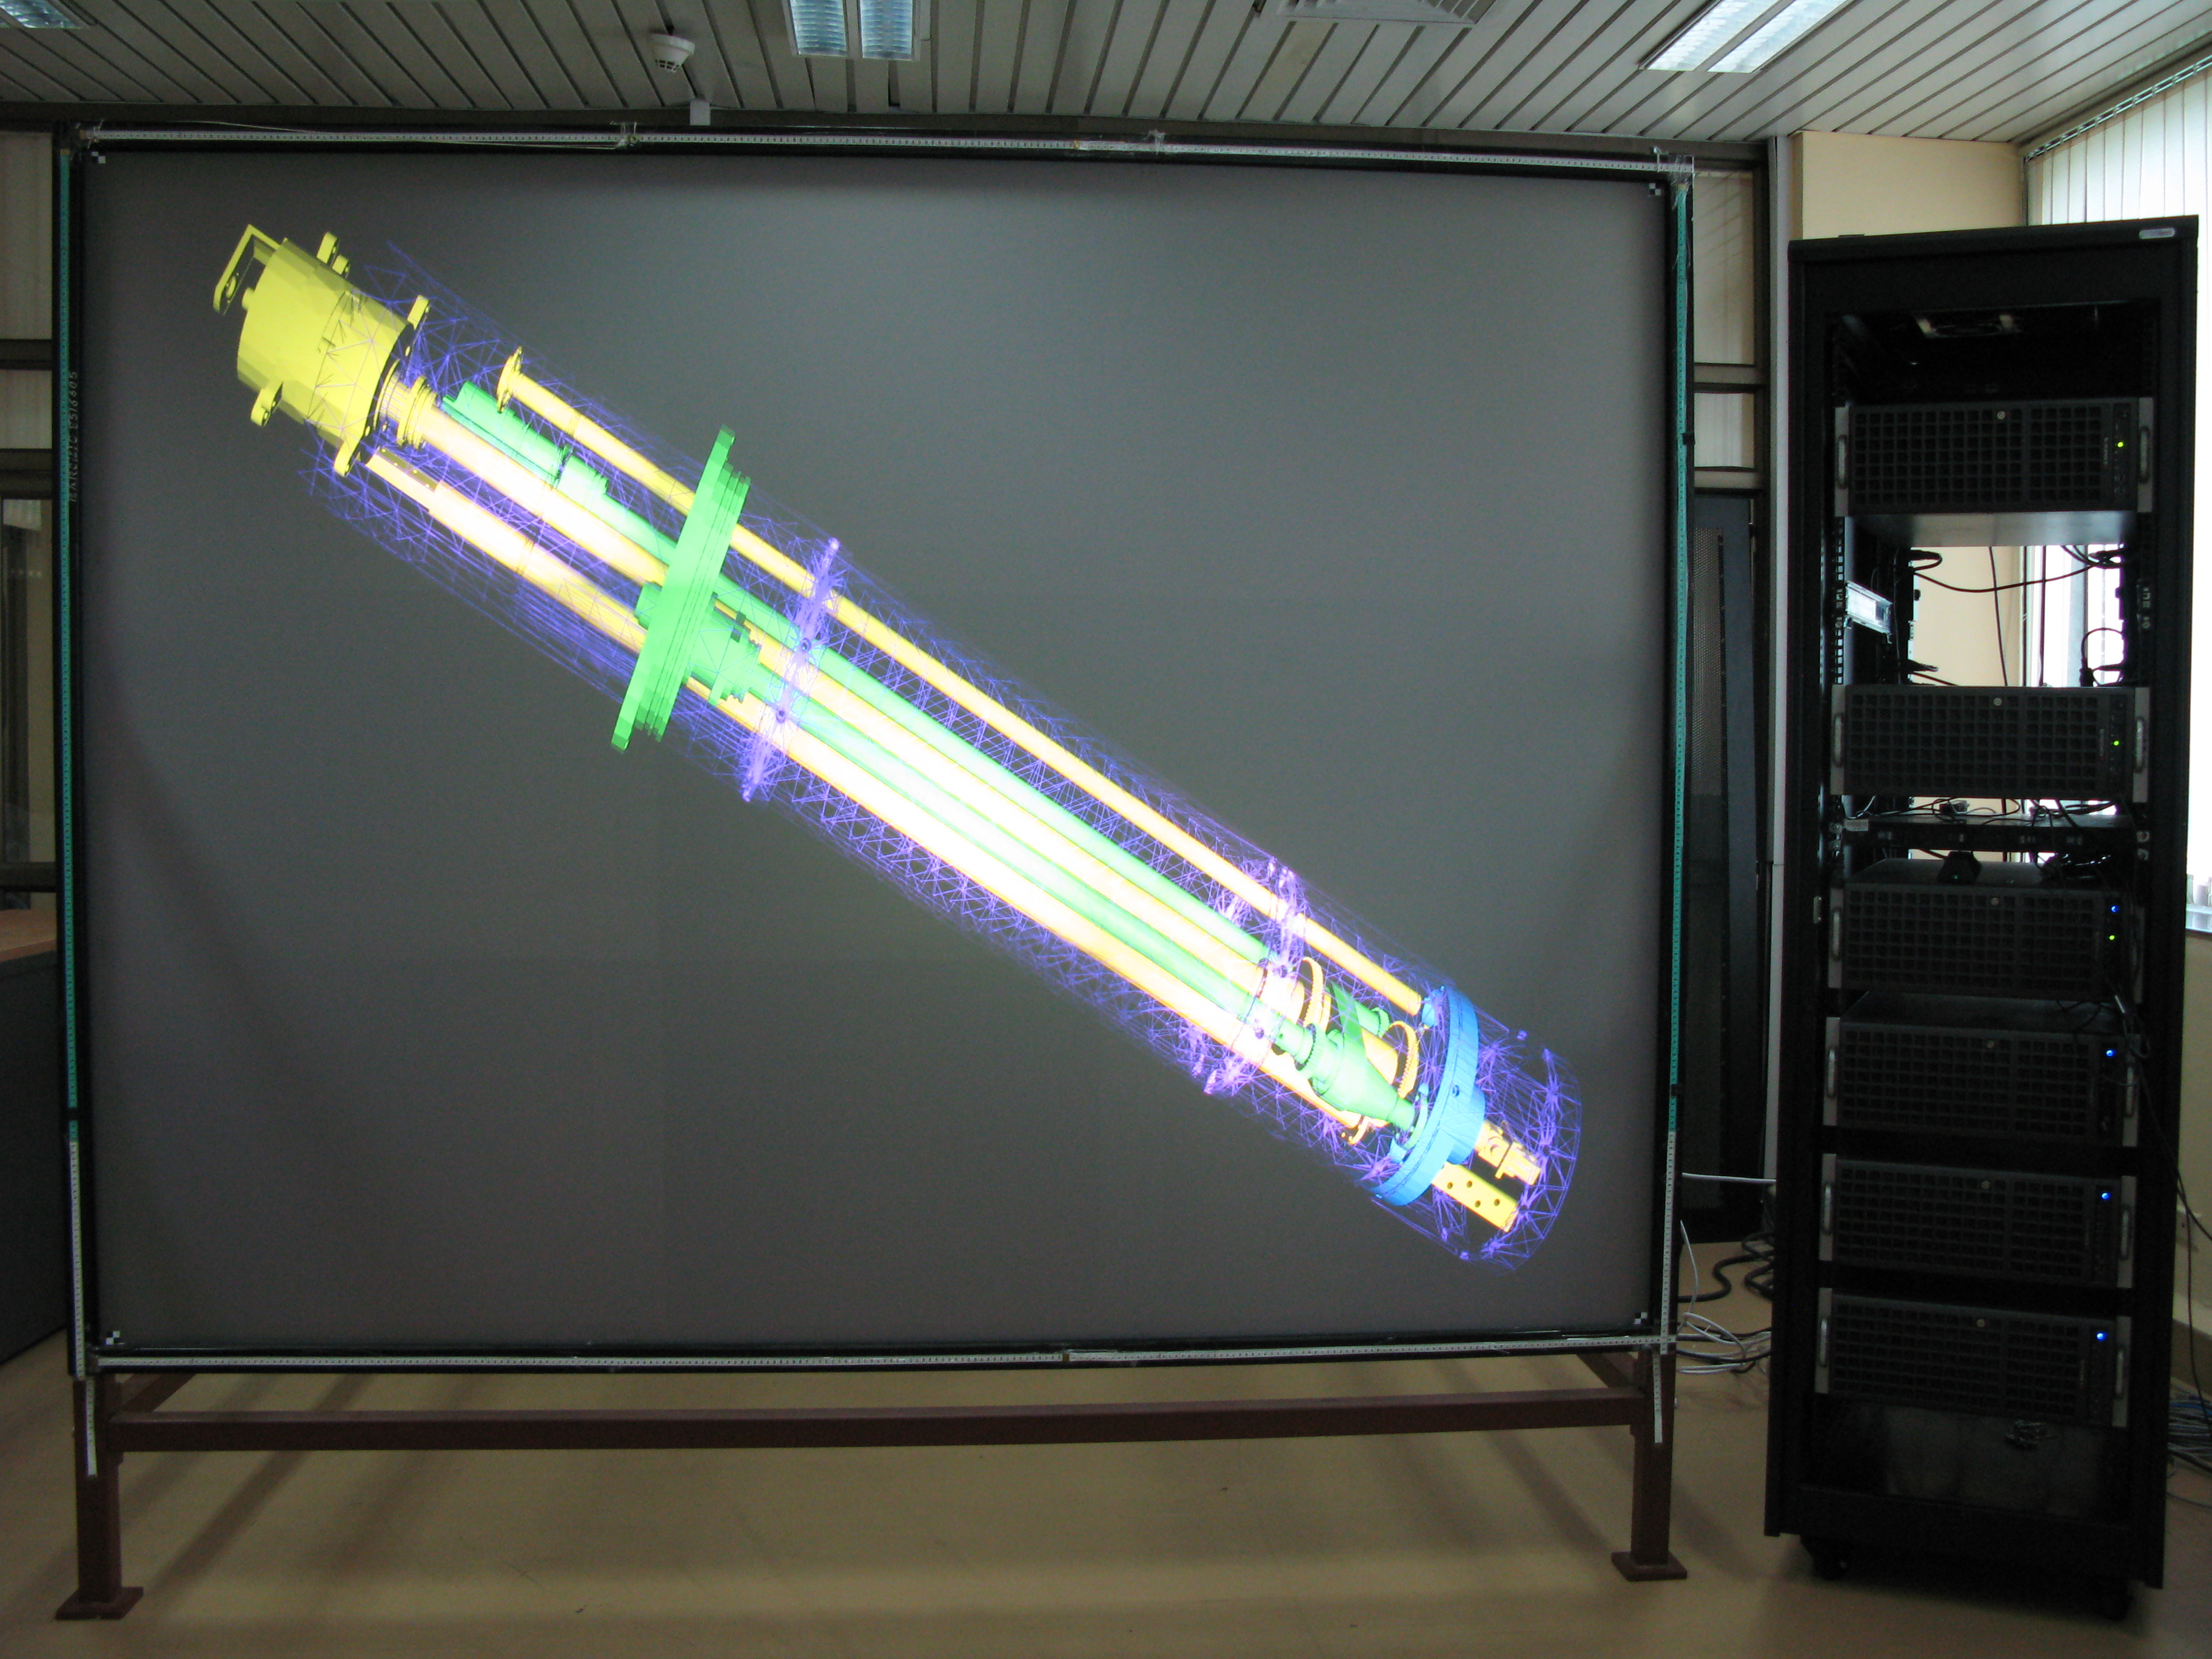
\includegraphics[width=5cm,height=3cm]{figures/3.JPG}} & 
\subfloat[]{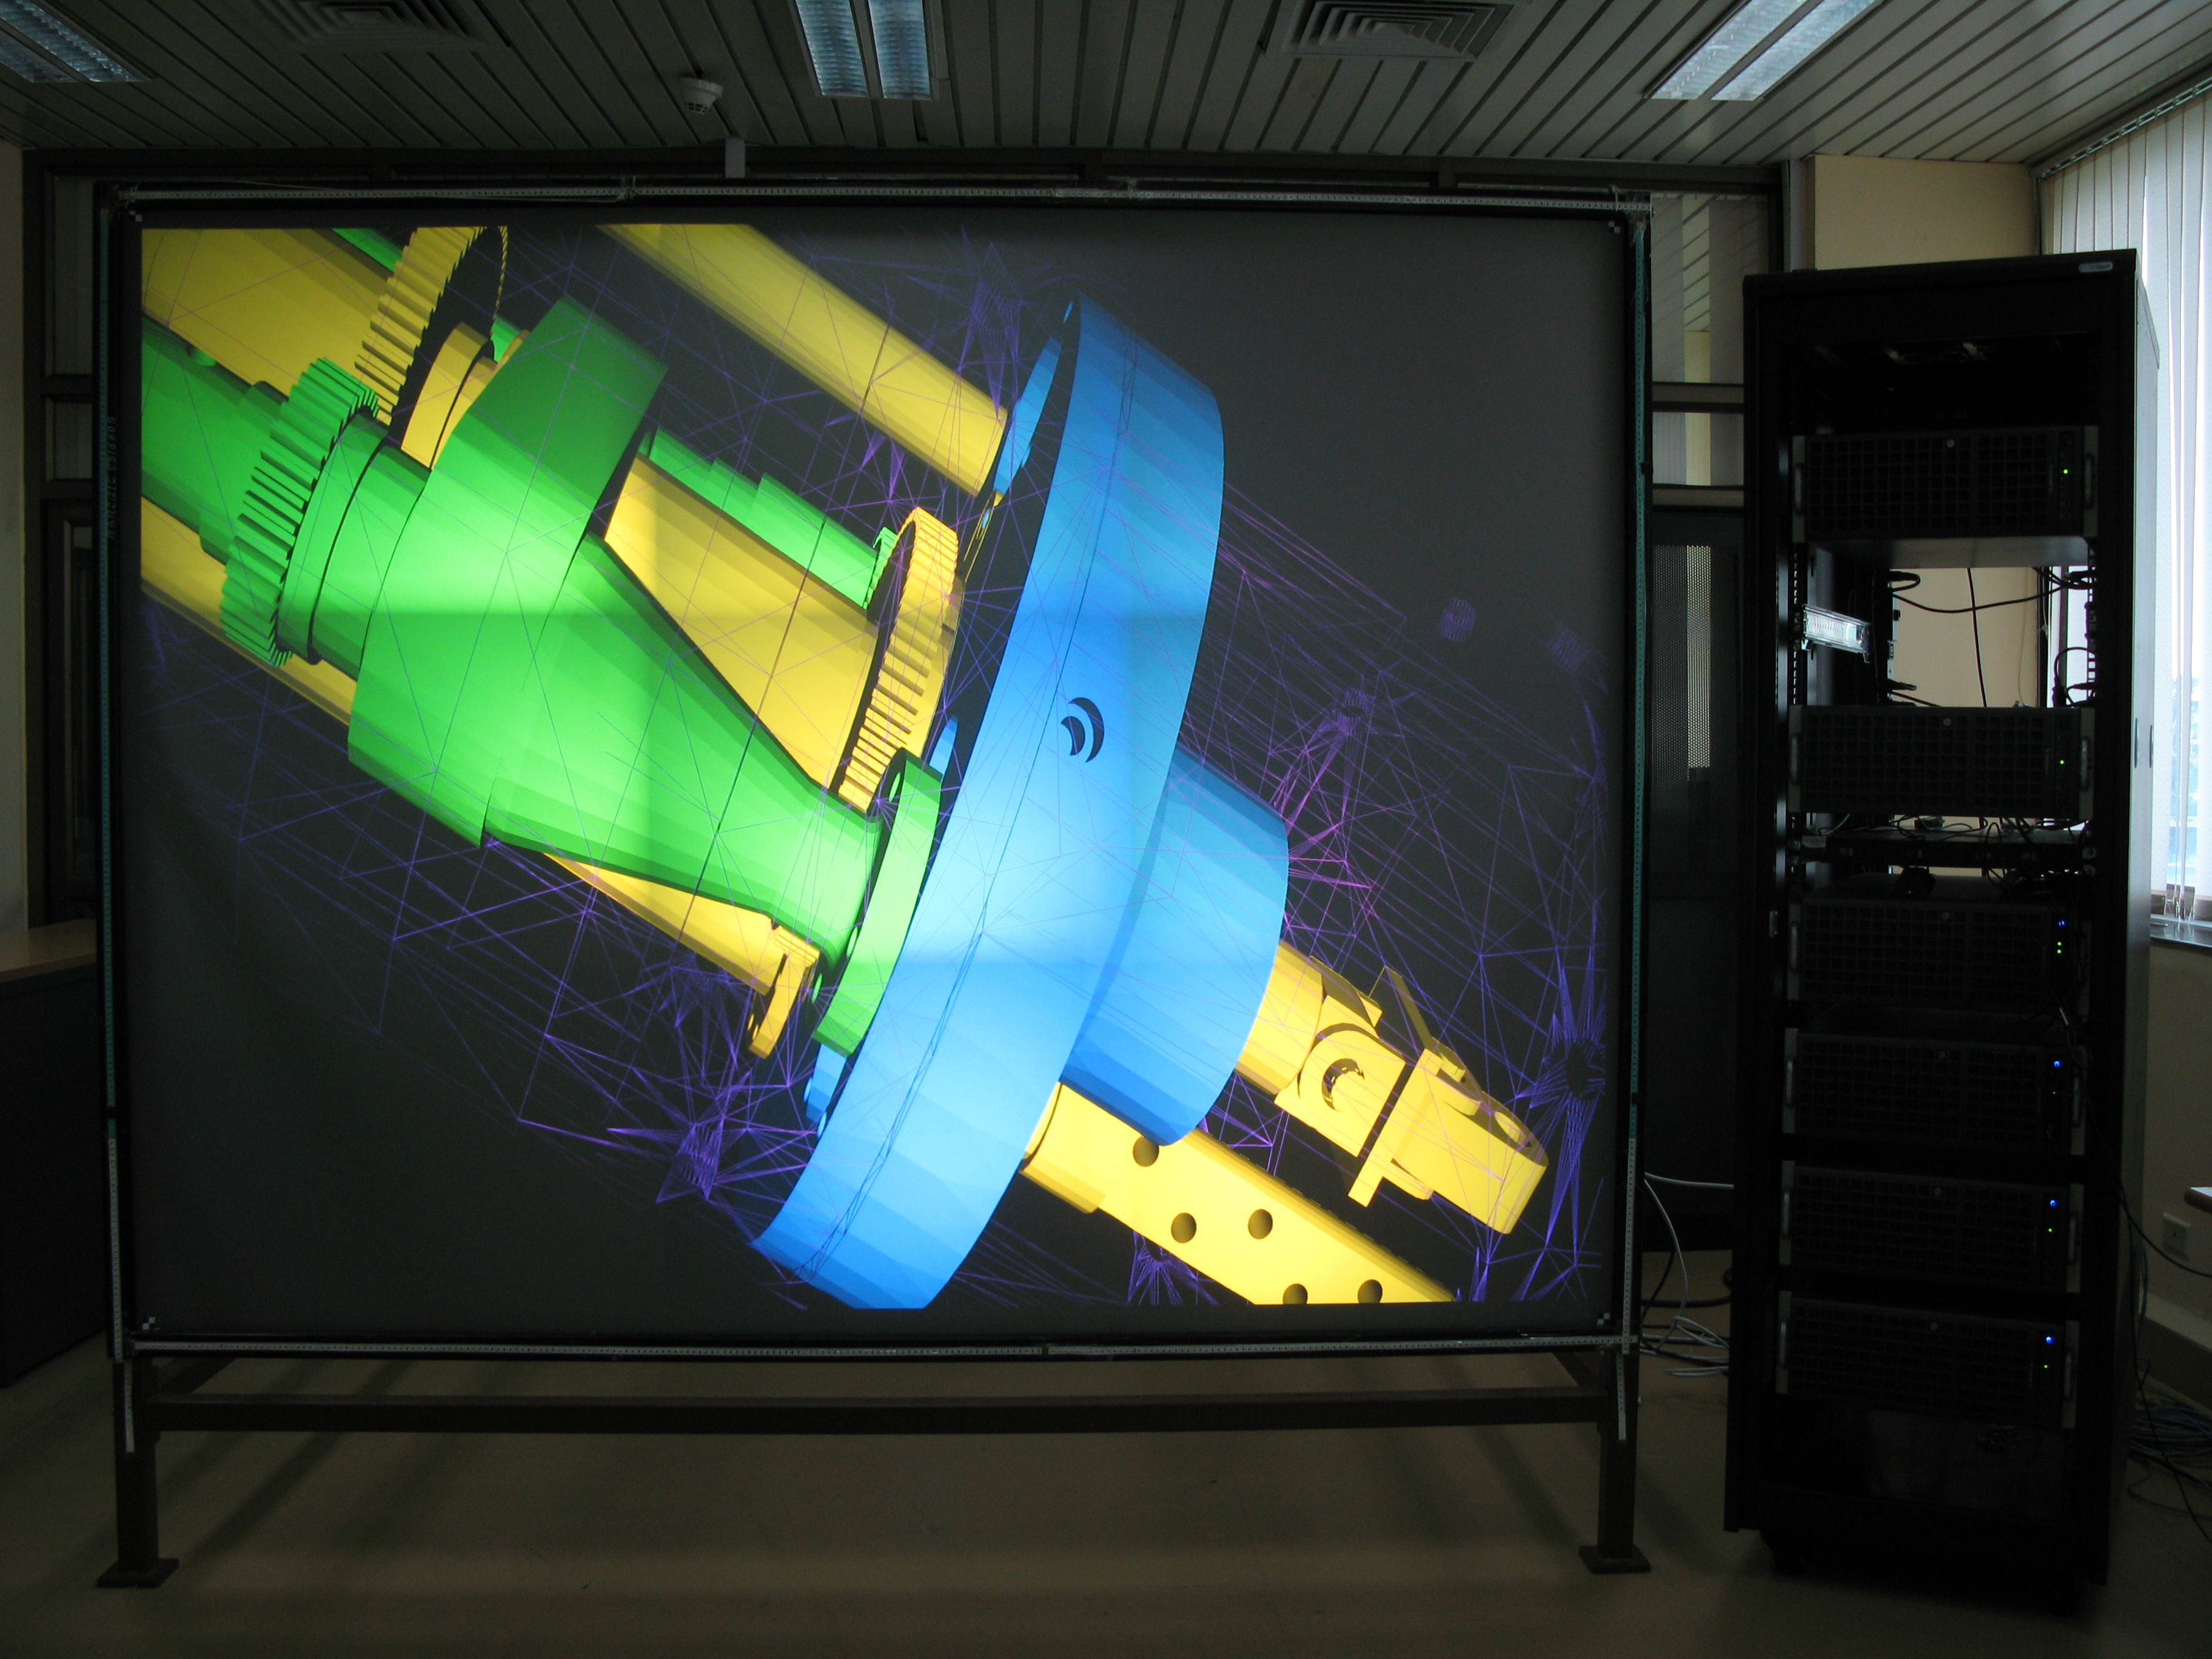
\includegraphics[width=5cm,height=3cm]{figures/4.JPG}} \\ 
\end{tabular}
\end{tabularx}
\end{figure}

\end{frame}



\begin{frame}{Thank you!!}
\begin{figure}
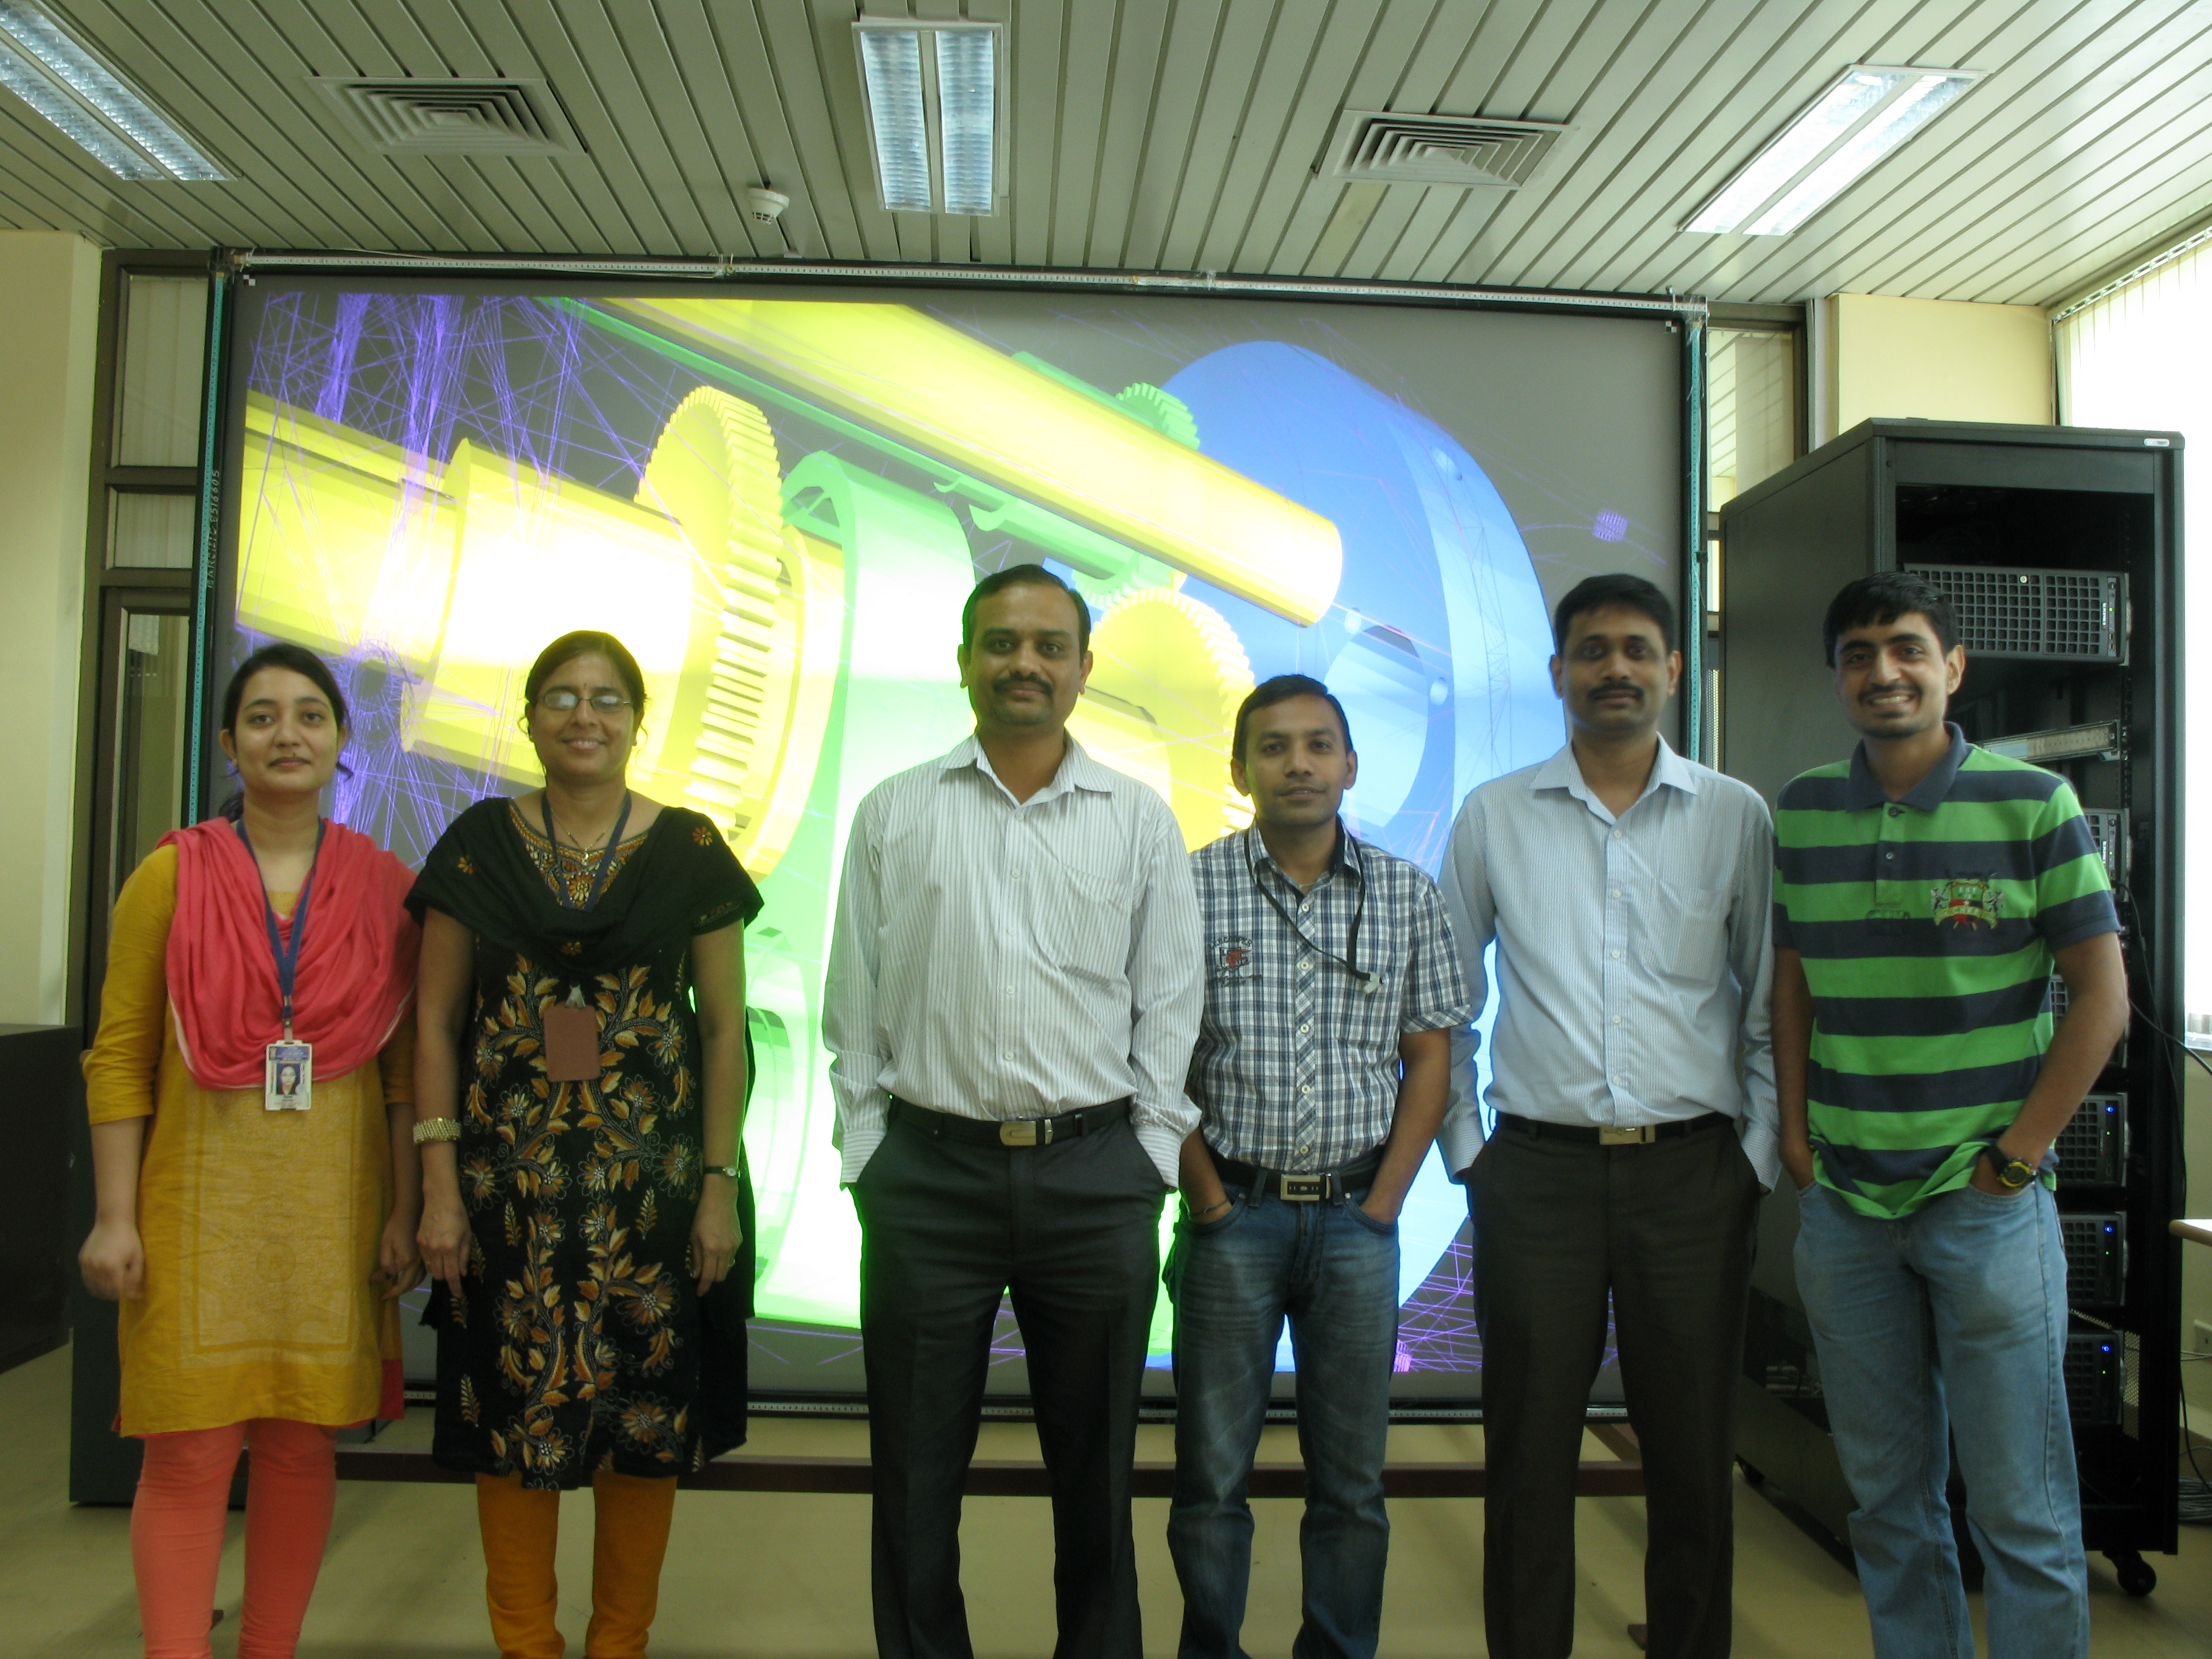
\includegraphics[width=\textwidth,height=\textheight]{figures/ThankYou.jpg}
\end{figure}
\end{frame}

%//////////////////////////////////////////////////////////////////////////////////////////////////////////////////////////////////

\appendix

%//////////////////////////////////////////////////////////////////////////////////////////////////////////////////////////////////

\begin{frame}[label=sysconfg]
\begin{itemize}
\item \underline{Software}:
\begin{itemize}
\item Written in C
\item Dependent on OpenCV(v2.4.1) and libgphoto2(v2.5.2)
\item Works on Ubuntu(12.04 LTS) and Scientific Linux(6.1)
\end{itemize}      
\item \underline{Hardware}:
\begin{itemize}
\item 3X3 grid of NEC 200X DLP projectors
\item 2.4mX1.8m acrylic glass based rear projection screen(from ScreenTech,Germany)
\item Canon Powershot G7 digital camera
\item 4 Workstations(1 master+ 3 slave) each with Intel® Xeon® Six Core Processor X5670, NVIDIA Quadro FX 4600 Graphics card and 48 GB ECC RAM.
\end{itemize}
\end{itemize}
\end{frame}

%//////////////////////////////////////////////////////////////////////////////////////////////////////////////////////////////////



\end{document}
